% \documentclass{article}
% \documentclass{book}
\documentclass{report} % Chọn cỡ chữ
\usepackage{Start}
\begin{document} % Bắt đầu

% \begin{titlepage}

    % Vẽ hình chữ nhật
    
    \begin{tikzpicture}[remember picture, overlay]\draw [line width = 3pt]($ (current page.north west) + (3.0cm, - 2.5cm)$)rectangle($ (current page.south east) + (- 2.5cm, 2.5cm)$);\draw [line width = 0.5pt]($ (current page.north west) + (3.1cm, - 2.6cm)$)rectangle($ (current page.south east) + (- 2.6cm, 2.6cm)$);\end{tikzpicture}
    
    \begin{center}
    
    \vspace{- 0.4cm}
    
    \textbf{ĐẠI HỌC BÁCH KHOA HÀ NỘI} \\
    
    \textbf{VIỆN TOÁN ỨNG DỤNG VÀ TIN HỌC} \\
    
    \textbf{******}
    
    \vspace{0.8cm}
    
    \begin{figure}[H]
    
    \centering
    
    
\includegraphics[scale = 0.5]{pictures/_hust/main.png}
    
    \end{figure}
    
    \vspace{0.7cm}
    
    \textbf{\fontsize{16pt}{30pt}\selectfont {BÁO CÁO ĐỒ ÁN II}}
    
    \vspace{1cm}
    
    \textbf{\fontsize{16pt}{30pt}\selectfont {ĐỀ TÀI:}} \\
    
    \textbf{\fontsize{20pt}{24pt}\selectfont {Sử dụng thiết kế hướng miền \\ xây dựng kiến trúc vi dịch vụ cho \\ bài toán hóa đơn điện tử}} \\
    
    \end{center}
    
    \vspace{0.3cm}
    
    \begin{center}
    
    \textbf{\fontsize{10pt}{24pt}\selectfont {Chuyên ngành: Toán Tin}}
    
    \end{center}
    
    \vspace{0.7cm}
    
    \hspace{3cm}\begin{minipage}{0.7\textwidth}
    
    \begin{tabular}{l l l}
    
    \textbf{\fontsize{10pt}{24pt}\selectfont {Giảng viên hướng dẫn}} & \textbf{\fontsize{10pt}{24pt}\selectfont {TS. Vũ Thành Nam}} \\
    
    \textbf{\fontsize{10pt}{24pt}\selectfont {Sinh viên thực hiện}} & \textbf{\fontsize{10pt}{24pt}\selectfont {Vũ Văn Nghĩa}} \\
    
    \textbf{\fontsize{10pt}{24pt}\selectfont {Mã số sinh viên}} & \textbf{\fontsize{10pt}{24pt}\selectfont {20206205}} \\
    
    \textbf{\fontsize{10pt}{24pt}\selectfont {Lớp}} & \textbf{\fontsize{10pt}{24pt}\selectfont {Toán Tin 02 - K65}} \\
    
    \end{tabular}
    
    \end{minipage}
    
    \vfill
    
    \begin{center}
    
    \textbf{Hà Nội, \the\year}
    
    % \textbf{Hà Nội, \the\month~/~\the\year}
    
    % \textbf{Hà Nội, \the\month~-~\the\year}
    
    \end{center}
    
    \end{titlepage}
    
    
% \begin{titlepage}

    % Vẽ hình chữ nhật
    
    \begin{tikzpicture}[remember picture, overlay]\draw [line width = 3pt]($ (current page.north west) + (3.0cm, - 2.5cm)$)rectangle($ (current page.south east) + (- 2.5cm, 2.5cm)$);\draw [line width = 0.5pt]($ (current page.north west) + (3.1cm, - 2.6cm)$)rectangle($ (current page.south east) + (- 2.6cm, 2.6cm)$);\end{tikzpicture}
    
    \begin{center}
    
    \vspace{- 0.4cm}
    
    \textbf{ĐẠI HỌC BÁCH KHOA HÀ NỘI} \\
    
    \textbf{VIỆN TOÁN ỨNG DỤNG VÀ TIN HỌC} \\
    
    \textbf{******}
    
    \vspace{0.8cm}
    
    \begin{figure}[H]
    
    \centering
    
    
\includegraphics[scale = 0.5]{pictures/_hust/main.png}
    
    \end{figure}
    
    \vspace{0.7cm}
    
    \textbf{\fontsize{16pt}{30pt}\selectfont {BÁO CÁO ĐỒ ÁN II}}
    
    \vspace{1cm}
    
    \textbf{\fontsize{16pt}{30pt}\selectfont {ĐỀ TÀI:}} \\
    
    \textbf{\fontsize{20pt}{24pt}\selectfont {Sử dụng thiết kế hướng miền \\ xây dựng kiến trúc vi dịch vụ cho \\ bài toán hóa đơn điện tử}} \\
    
    \end{center}
    
    \vspace{0.3cm}
    
    \begin{center}
    
    \textbf{\fontsize{10pt}{24pt}\selectfont {Chuyên ngành: Toán Tin}}
    
    \end{center}
    
    \vspace{0.7cm}
    
    \hspace{3cm}\begin{minipage}{0.7\textwidth}
    
    \begin{tabular}{l l l}
    
    \textbf{\fontsize{10pt}{24pt}\selectfont {Giảng viên hướng dẫn}} & \textbf{\fontsize{10pt}{24pt}\selectfont {TS. Vũ Thành Nam}} \\
    
    \textbf{\fontsize{10pt}{24pt}\selectfont {Sinh viên thực hiện}} & \textbf{\fontsize{10pt}{24pt}\selectfont {Vũ Văn Nghĩa}} \\
    
    \textbf{\fontsize{10pt}{24pt}\selectfont {Mã số sinh viên}} & \textbf{\fontsize{10pt}{24pt}\selectfont {20206205}} \\
    
    \textbf{\fontsize{10pt}{24pt}\selectfont {Lớp}} & \textbf{\fontsize{10pt}{24pt}\selectfont {Toán Tin 02 - K65}} \\
    
    \end{tabular}
    
    \end{minipage}
    
    \vfill
    
    \begin{center}
    
    \textbf{Hà Nội, \the\year}
    
    % \textbf{Hà Nội, \the\month~/~\the\year}
    
    % \textbf{Hà Nội, \the\month~-~\the\year}
    
    \end{center}
    
    \end{titlepage}
    
    
% \begin{center}

    {\bfseries NHẬN XÉT CỦA GIẢNG VIÊN HƯỚNG DẪN}
    
    \end{center}
    
    \begin{enumerate}
    
    \item Mục đích và nội dung của đồ án:
    
    \vspace{20ex}
    
    \item Kết quả đạt được:
    
    \vspace{20ex}
    
    \item Ý thức làm việc của sinh viên:
    
    \vspace{20ex}
    
    \end{enumerate}
    
    \hspace{0.4\textwidth}\begin{minipage}{0.5\textwidth}
    
    \noindent\begin{center}
    
    \textit{Hà Nội, \today} \\
    
    \textbf{Giảng viên hướng dẫn} \\
    
    \textit{(Ký và ghi rõ họ tên)}
    
    \vspace{2cm}
    
    \textbf{TS. Vũ Thành Nam}
    
    \end{center}
    
    \end{minipage}
    
    \pagestyle{empty}
    
    
% 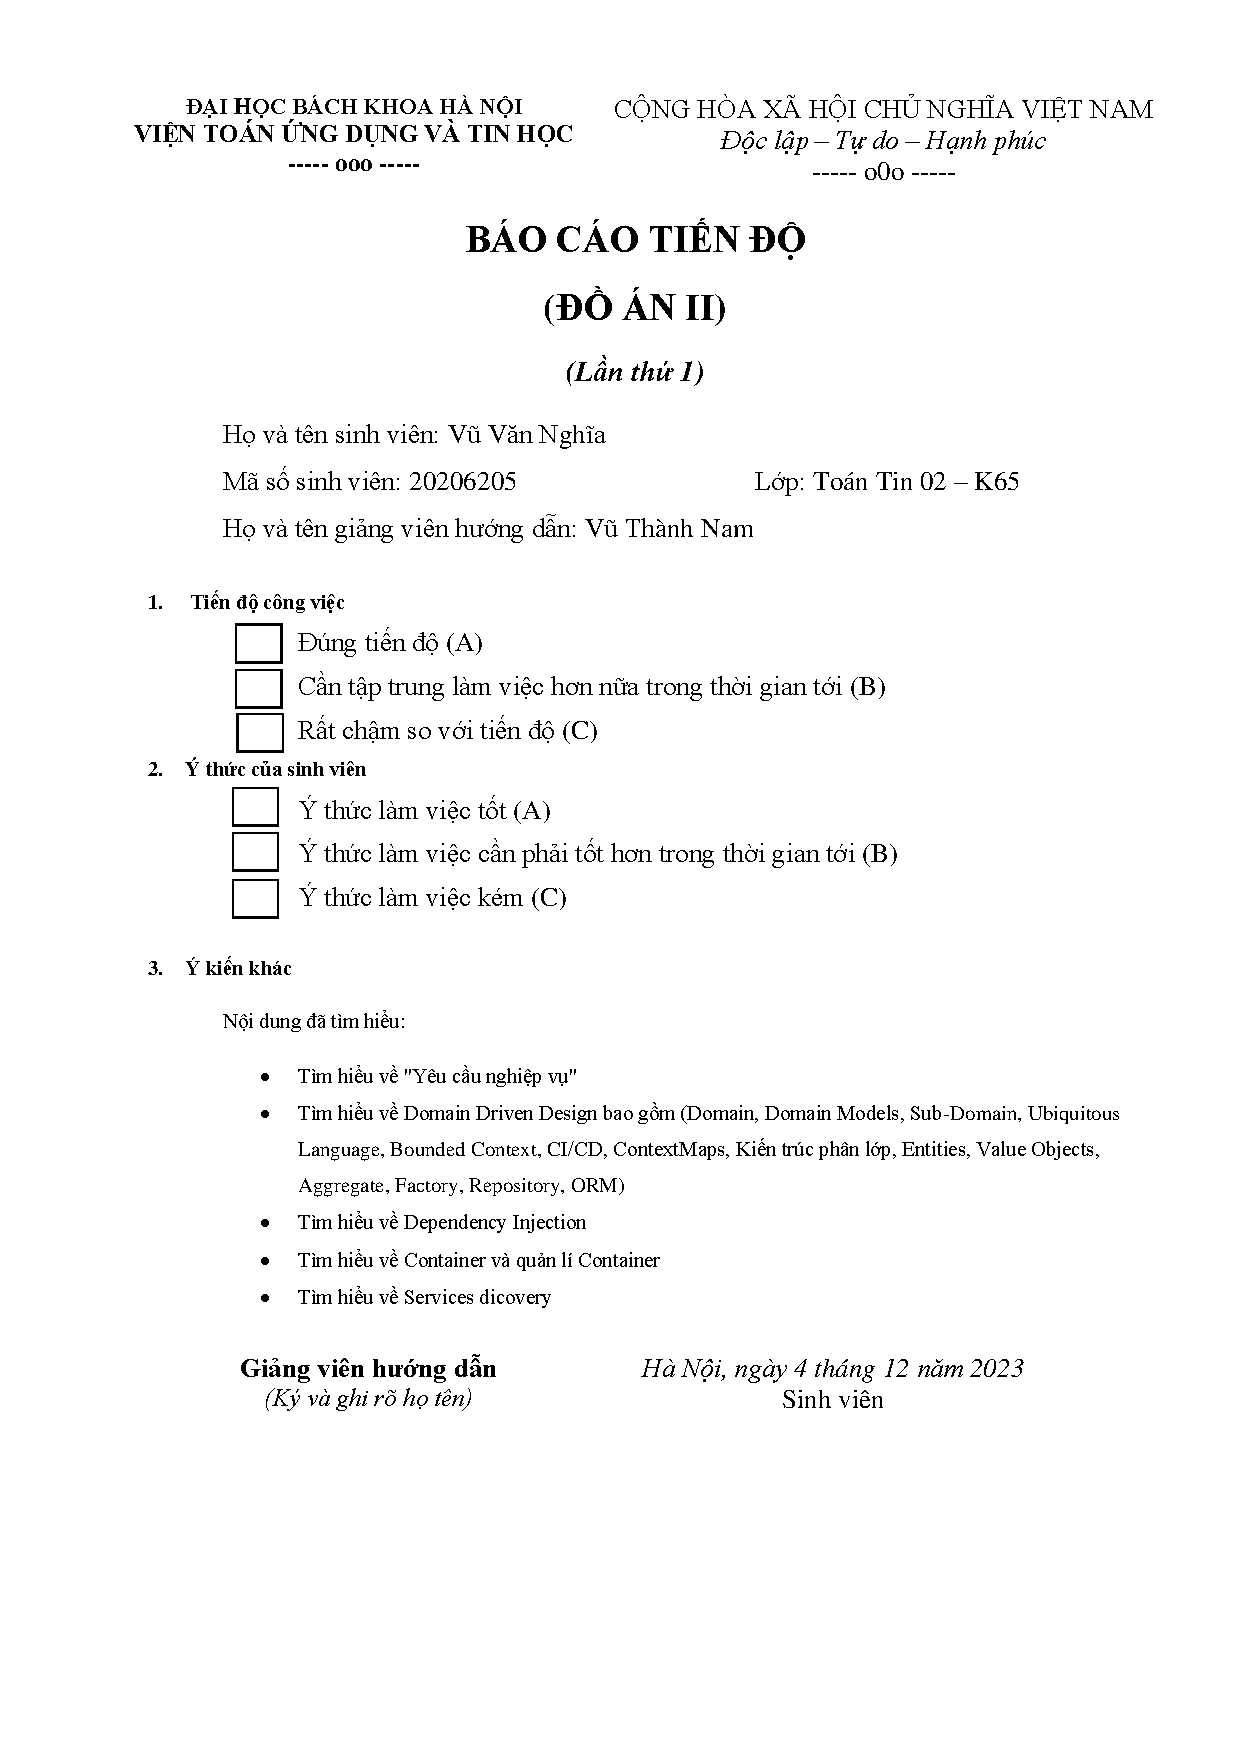
\includepdf[pages = -]{contents/bao_cao_tien_do/lan_1.pdf}
% 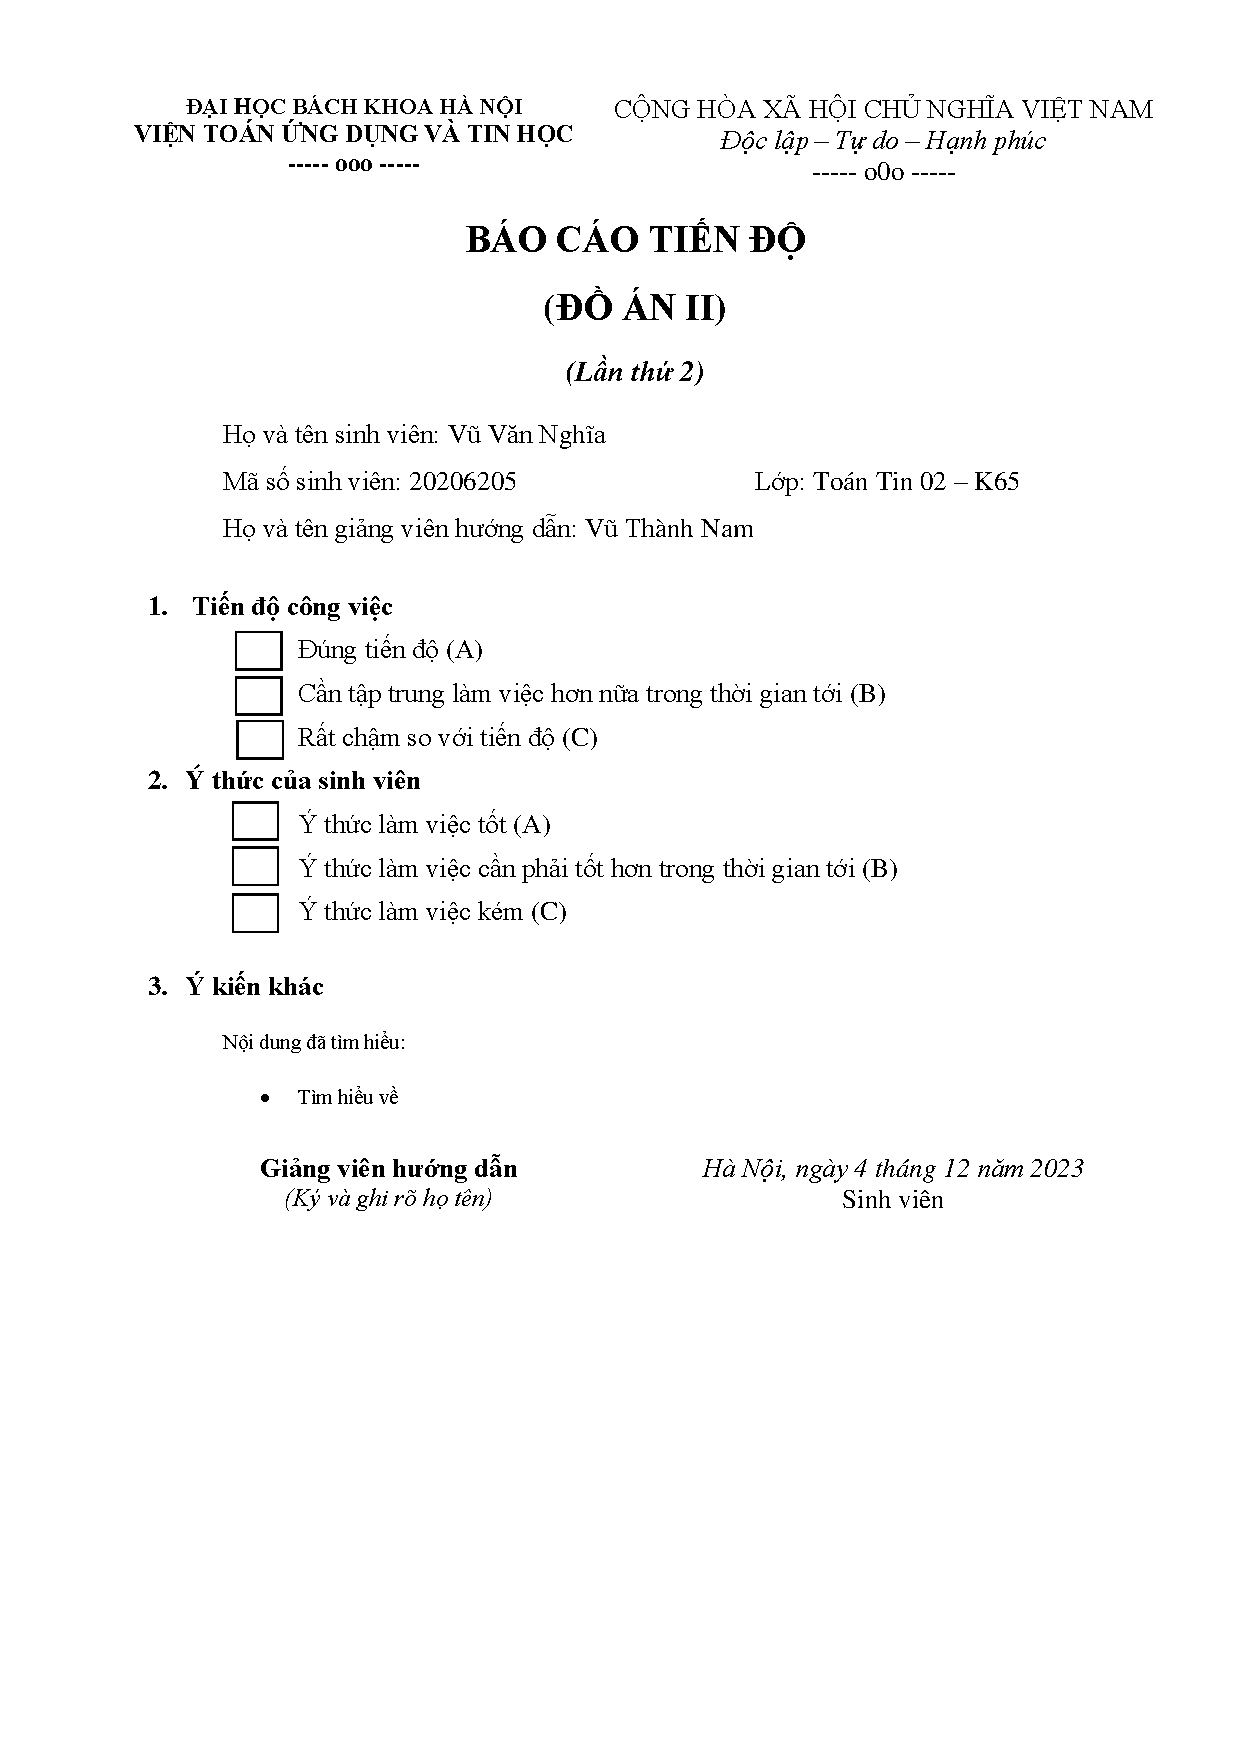
\includepdf[pages = -]{contents/bao_cao_tien_do/lan_2.pdf}
% \renewcommand*\contentsname{\centering MỤC LỤC}

\tableofcontents

\setcounter{page}{0}


% \chapter*{\centering LỜI CẢM ƠN}

\addcontentsline{toc}{chapter}{LỜI CẢM ƠN}

Trước hết, em xin gửi lời cảm ơn chân thành và sâu sắc đến TS. Vũ Thành Nam, người thầy đã tận tình hỗ trợ và hướng dẫn em suốt thời gian thực hiện đồ án. Những kiến thức và kinh nghiệm mà em đã tiếp thu được trong quá trình này sẽ đóng góp quan trọng vào sự phát triển và thành công của em trong tương lai. Em xin gửi lời chúc sức khỏe tốt nhất đến thầy, hy vọng thầy luôn dồi dào sức khỏe, đam mê và nhiệt huyết trong công việc giảng dạy.

Em cũng xin gửi lời cảm ơn tới các thầy cô giảng viên trong \emph{"Khoa Toán - Tin"} đã tận tình truyền đạt những kiến thức quý báu cho em. Những kiến thức này không chỉ giúp em phát triển về mặt tri thức mà còn nuôi dưỡng kỹ năng và đam mê trong quá trình học tập và nghiên cứu.

Trong quá trình hoàn thành bài báo cáo đồ án này không tránh khỏi những thiếu sót. Vì vậy, em mong nhận được sự giúp đỡ và ý kiến đóng góp chân thành từ các thầy cô để em có thể cải thiện một cách tốt nhất.

\emph{Em xin chân thành cảm ơn!}

\vspace{0.7cm}

\hspace{0.4\textwidth}\begin{minipage}{0.5\textwidth}

\noindent\begin{center}

\textit{Hà Nội, \today} \\

\vspace{0.5cm}

\textbf{Tác giả} \\

\vspace{0.5cm}

\textbf{Vũ Văn Nghĩa}

\end{center}

\end{minipage}
% \chapter*{\centering DANH SÁCH BẢNG}

\addcontentsline{toc}{chapter}{DANH SÁCH BẢNG}

\makeatletter

\renewcommand\listoftables{

\@starttoc{lot}

}

\makeatother

\listoftables
% \chapter*{\centering DANH SÁCH HÌNH ẢNH}

\addcontentsline{toc}{chapter}{DANH SÁCH HÌNH ẢNH}

\makeatletter

\renewcommand\listoffigures{

\@starttoc{lof}

}

\makeatother

\listoffigures
% %%%%%%%%%%%%%%%%%%%%%%%%%%%%%%

%%%%%%%%%%%%%%%%%%%%%%%%%%%%%%

\chapter*{\centering DANH SÁCH CÁC CỤM TỪ VIẾT TẮT}

\addcontentsline{toc}{chapter}{DANH SÁCH CÁC CỤM TỪ VIẾT TẮT}

% @sau

% @sau

% @sau

% @sau

% @sau

% @sau

% @sau

% @sau

% @sau

% @sau

% @sau

% @sau

% @sau

% @sau

% @sau

% @sau

% @sau

% @sau

% @sau

% @sau

% @sau

% @sau

% @sau

% @sau

% @sau

% @sau

% @sau

% @sau

% @sau

% @sau

\begin{table}[h]

\centering

\begin{tabular}{|c|c|c|c|}

\hline

STT & Từ viết tắt & Từ viết đầy đủ & Mô tả \\

\hline

Dong1 & Dong1 & Cot1 & Cot2 \\

\hline

Dong2 & Dong2 & Cot1 & Cot2 \\

\hline

\end{tabular}

\end{table}

% API; Application Programming Interface; Giao diện lập trình ứng dụng

% CI/CD; Continuous Integration (CI) and Continuous Delivery (CD) ; Quá trình tích hợp và chuyển giao liên tục

% thiết kế hướng miền ; thiết kế hướng miền; Kỹ thuật thiết kế theo hướng miền

% DI; Dependency Injection; Cơ chế tiêm sự phụ thuộc giữa các đối tượng

% HTTP; Hypertext Transfer Protocol; Giao thức truyền tải siêu văn bản

% JSON; JavaScript Object Notation; Một kiểu dữ liệu mở rộng của JavaScript

% ORM; Object Relational Mapping; Một kỹ thuật ánh xạ các đối tượng lập trình với từng bảng trong CSDL quan hệ

% Cơ sở dữ liệu ; CSDL ;

% Tạo (Create), Đọc (Read), Sửa (Update), Xóa (Delete) ; CRUD ;

% Kubernetes ; K8s ; kubernetes

% Số điện thoại ; SĐT ;

% UML

% MVC; Model View Controller; Một mẫu thiết kế ứng dụng

% SQL

SOA; Service Oriented Architecture; Kiến trúc hướng dịch vụ

SOAP; Simple Object Access Protocol; Một giao thức để truy cập dịch vụ web

SPA; Single Page Application; Kiểu ứng dụng một trang

REST; Representational State Transfer; Một tiêu chuẩn thiết kế các API sử dụng cho các dịch vụ web

URL; Uniform Resource Locator ; Địa chỉ định vị tài nguyên trên Internet

XML; Extensible Markup Language; Ngôn ngữ đánh dấu mở rộng

% TCT ; TCT ;

Người nộp thuế ; NNT ;

Mã số thuế ; MST ;

Hóa đơn điện tử ; HĐĐT ;

Cơ quan thuế ; CQT ;

Công nghệ thông tin ; CNTT ;

%%%%%%%%%%%%%%%%%%%%%%%%%%%%%%
% \chapter*{\centering DANH SÁCH CÁC THUẬT NGỮ}

\addcontentsline{toc}{chapter}{DANH SÁCH CÁC THUẬT NGỮ}

% @sau

% @sau

% @sau

% @sau

% @sau

% @sau

% @sau

% @sau

% @sau

% @sau

% @sau

% @sau

% @sau

% @sau

% @sau

% @sau

% @sau

% @sau

% @sau

% @sau

% @sau

% @sau

% @sau

% @sau

% @sau

% @sau

% @sau

% @sau

\begin{table}[h]

\centering

\begin{tabular}{|c|c|c|}

\hline

STT & Tiếng Anh & Tiếng Việt \\

\hline

Dong1 & Dong1 & Cot2 \\

\hline

Dong2 & Dong2 & Cot2 \\

\hline

\end{tabular}

\end{table}

% kiến trúc nguyên khối, kiến trúc nguyên khối

% kiến trúc nguyên khối, kiến trúc nguyên khối

% kiến trúc vi dịch, kiến trúc vi dịch

% kiến trúc vi dịch, kiến trúc vi dịch

% kiến trúc vi dịch, kiến trúc vi dịch

% kiến trúc vi dịch, kiến trúc vi dịch

% thiết kế hướng miền, thiết kế hướng miền

% thiết kế hướng miền, thiết kế hướng miền

1 thiết kế hướng miền

Thiết kế hướng lĩnh vực

2 Domain (không dịch)

3 Abstraction Trừu tượng

4 chuyên gia ngành

% \chapter*{\centering MỞ ĐẦU}
% \addcontentsline{toc}{chapter}{MỞ ĐẦU}
% \section*{Lý do chọn đề tài}
% Trong quá trình hoạt động kinh doanh, doanh nghiệp có nhu cầu chuyển đổi mô hình kinh doanh linh hoạt để có thể tồn tại và phát triển khi thị trường thay đổi. Từ đó, đáp ứng nhu cầu của khách hàng, mang lại ưu thế cạnh tranh so với các đối thủ.

Trong những năm gần đây, việc áp dụng kiến trúc vi dịch vụ ngày càng phổ biến, đem lại nhiều lợi ích như tách các nghiệp vụ kinh doanh thành các dịch vụ nhỏ độc lập, tăng tính linh hoạt và khả năng chống chịu sự cố của hệ thống.

Kiến trúc vi dịch vụ hỗ trợ doanh nghiệp chuyển đổi nhanh chóng để đáp ứng nhu cầu của mô hình kinh doanh và mong đợi của khách hàng. Tuy nhiên, để xây dựng được kiến trúc vi dịch vụ tốt, cần phải tạo ra các dịch vụ nhỏ phù hợp và duy trì tính độc lập. Trong đồ án này, em sử dụng thiết kế hướng miền để phân tích và xây dựng kiến trúc vi dịch vụ.

Theo quy định của Nghị định 123/2020/NĐ - CP, tất cả các doanh nghiệp, tổ chức và hộ kinh doanh đều bắt buộc phải sử dụng hóa điện tử. Vì vậy, nhu cầu sử dụng và xử lý hóa đơn điện tử trở nên rất lớn. Do đó trong đồ án này, em chọn chủ đề \emph{"Sử dụng thiết kế hướng miền xây dựng kiến trúc vi dịch vụ cho bài toán hóa đơn điện tử"}. Chủ đề này là một xu hướng quan trọng trong phát triển phần mềm và mang lại nhiều lợi ích trong việc cải thiện quá trình quản lý hóa đơn điện tử.
% \section*{Đối tượng và phạm vi nghiên cứu}
% \begin{itemize}

\item \textbf{Đối tượng nghiên cứu:} Kiến trúc vi dịch vụ

\item \textbf{Phạm vi nghiên cứu:} Tập trung vào tìm hiểu thiết kế hướng miền xây dựng kiến trúc vi dịch vụ cho bài toán hóa đơn điện tử.

\end{itemize}


% \section*{Tóm tắt nội dung đồ án}
% Báo cáo đồ án này được tổ chức thành các phần chính sau:

\begin{itemize}

    \item \textbf{Chương 1: xxxxxxxxxxxxxxxxx}

    \begin{quote}
    
        xxxxxxxxxxxxxxxxx
    
    \end{quote}  
    \item \textbf{Chương 1: xxxxxxxxxxxxxxxxx}
    
    \begin{quote}
    
        xxxxxxxxxxxxxxxxx
    
    \end{quote}  
    \item \textbf{Chương 1: xxxxxxxxxxxxxxxxx}
    
    \begin{quote}
    
        xxxxxxxxxxxxxxxxx
    
    \end{quote}  

\end{itemize}

%@ Thêm các mục nhỏ như:

%@ Thêm các mục nhỏ như:

%@ Thêm các mục nhỏ như:

%@ Thêm các mục nhỏ như:

%@ Thêm các mục nhỏ như:

%@ Thêm các mục nhỏ như:

%@ Thêm các mục nhỏ như:

%@ Thêm các mục nhỏ như:

%@ Thêm các mục nhỏ như:

%@ Thêm các mục nhỏ như:

%@ Thêm các mục nhỏ như:

%@ Thêm các mục nhỏ như:

%@ Thêm các mục nhỏ như:

% Luận văn được tổ chức thành các phần chính sau:

% Mở đầu: Trình bày tổng quan về đề tài

% Chương 1: Trình bày cách thức phát triển phần mềm theo kiến trúc kiến trúc vi dịch vụ .

% Trong chương này, luận văn tập trung làm rõ các nội dung:

% - Sơ lược về một số hướng kiến trúc phần mềm truyền thống như kiến trúc nguyên

% khối, kiến trúc hướng dịch vụ, công nghệ ESB

% - Tổng quan về kiến trúc kiến trúc vi dịch vụ : sự ra đời, đặc điểm của kiến trúc vi dịch vụ

% - Các mẫu thiết kế quan trọng được sử dụng trong kiến trúc vi dịch vụ

% - Một số nguyên tắc thiết kế kiến trúc vi dịch vụ

% Chương 2: Trình bày hướng xây dựng ứng dụng web sử dụng micro - frontends.

% Trong chương này, luận văn tập trung làm rõ các nội dung:

% - Sơ lược về một số mô hình phát triển web như mô hình web tĩnh, mô hình web

% động, mô hình web theo hướng SPA

% - Sự ra đời của kiến trúc micro - frontends

% - Các cơ chế tích hợp micro - frontends được thảo luận như: tích hợp theo hướng

% “build - time”, tích hợp theo hướng “run - time”, cách thức điều hướng và giao tiếp

% giữa các micro - frontends

% Chương 3: Trình bày cách thức xây dựng một ứng dụng thử nghiệm sử dụng kiến

% trúc kiến trúc vi dịch vụ, micro - frontends. Một số nội dung chính trong quá trình thực nghiệm

% được làm rõ bao gồm:

% 3

% - Áp dụng phương pháp thiết kế hướng miền để phân hoạch, thiết kế chương trình

% - Thiết kế và cài đặt tầng dịch vụ theo hướng kiến trúc vi dịch vụ, sử dụng các công

% nghệ trên nền tảng Java như Spring Boot, Spring Cloud

% - Thiết kế và cài đặt tầng giao diện theo hướng micro - frontends, sử dụng các công

% nghệ như Single - SPA, Angular, ReactJS

% - Một số kỹ thuật kiểm thử kiến trúc vi dịch vụ cũng được thảo luận như kiểm thử đơn

% vị, kiểm thử tích hợp và kiểm thử mức giao diện

% - Cách thức triển khai ứng dụng sử dụng Docker

% Phần kết luận: Tổng kết, đánh giá kết quả thu được của quá trình nghiên cứu cũng

% như các ưu nhược điểm, các hạn chế và hướng phát triển tương lai.

\chapter{Tổng quan về bài toán hóa đơn điện tử}
% Bài toán hóa đơn điện tử là một phần quan trọng của quá trình chuyển đổi số. Trong quá khứ, mọi người thường sử dụng hóa đơn giấy truyền thống. Ngày nay, khi có quy định kế toán và quản lý tài chính, hóa đơn điện tử đã trở nên phổ biến giúp giảm bớt sự phụ thuộc vào giấy tờ. Cùng với sự phát triển của khoa học công nghệ đã giúp quản lý hiệu quả công việc và tối ưu hóa quy trình kế toán và tài chính.
% \section{Các khái niệm và căn cứ pháp lý}
% \emph{Theo em tìm hiểu có các khái niệm và căn cứ pháp lý liên quan sau đây:}

\subsection{Hóa đơn}

\emph{Theo quy định tại khoản 1 Điều 3 Nghị định 123/2020/NĐ - CP:}

%%%%%%%%%%%%%%%%%%%%%%%%%%%%%%%%%%%%%!

Hóa đơn là chứng từ kế toán do tổ chức, cá nhân bán hàng hóa, cung cấp dịch vụ lập, ghi nhận thông tin bán hàng hóa, cung cấp dịch vụ. Hóa đơn được thể hiện theo hình thức hóa đơn điện tử hoặc hóa đơn do cơ quan thuế đặt in.

%%%%%%%%%%%%%%%%%%%%%%%%%%%%%%%%%%%%%!

\subsection{Hóa đơn điện tử}

\emph{Theo quy định tại khoản 2 Điều 3 Nghị định 123/2020/NĐ - CP:}

%%%%%%%%%%%%%%%%%%%%%%%%%%%%%%%%%%%%%!

Hóa đơn điện tử là hóa đơn có mã hoặc không có mã của cơ quan thuế được thể hiện ở dạng dữ liệu điện tử do tổ chức, cá nhân bán hàng hóa, cung cấp dịch vụ lập bằng phương tiện điện tử để ghi nhận thông tin bán hàng hóa, cung cấp dịch vụ theo quy định của pháp luật về kế toán, pháp luật về thuế, bao gồm cả trường hợp hóa đơn được khởi tạo từ máy tính tiền có kết nối chuyển dữ liệu điện tử với cơ quan thuế, trong đó:

a. Hóa đơn điện tử có mã của cơ quan thuế là hóa đơn điện tử được cơ quan thuế cấp mã trước khi tổ chức, cá nhân bán hàng hóa, cung cấp dịch vụ gửi cho người mua. Mã của cơ quan thuế trên hóa đơn điện tử bao gồm số giao dịch là một dãy số duy nhất do hệ thống của cơ quan thuế tạo ra và một chuỗi ký tự được cơ quan thuế mã hóa dựa trên thông tin của người bán lập trên hóa đơn.

b. Hóa đơn điện tử không có mã của cơ quan thuế là hóa đơn điện tử do tổ chức bán hàng hóa, cung cấp dịch vụ gửi cho người mua không có mã của cơ quan thuế.

%%%%%%%%%%%%%%%%%%%%%%%%%%%%%%%%%%%%%!

\subsection{Bắt buộc sử dụng hóa đơn điện tử từ 01/07/2022}

\emph{Theo quy định tại khoản 1 Điều 59 Nghị định 123/2020/NĐ - CP:}

%%%%%%%%%%%%%%%%%%%%%%%%%%%%%%%%%%%%%!

Nghị định này có hiệu lực thi hành kể từ ngày 01 tháng 7 năm 2022, khuyến khích cơ quan, tổ chức, cá nhân đáp ứng điều kiện về hạ tầng công nghệ thông tin áp dụng quy định về hóa đơn, chứng từ điện tử của Nghị định này trước ngày 01 tháng 7 năm 2022.

%%%%%%%%%%%%%%%%%%%%%%%%%%%%%%%%%%%%%!

% Chủ đề đồ án

$\Rightarrow$ Theo quy định, tất cả các doanh nghiệp, tổ chức và hộ kinh doanh đều bắt buộc phải chuyển từ sử dụng hóa đơn giấy sang hóa đơn điện tử bắt đầu từ tháng 07/2022. Vì vậy, nhu cầu sử dụng và xử lý hóa đơn điện tử trở nên rất lớn. Do đó ở đồ án này, em chọn chủ đề về quản lý hóa đơn điện tử.

\subsection{Qui định lưu trữ hóa đơn điện tử}

\emph{Theo quy định tại khoản 1 Điều 11 Thông tư 32/2011/TT - BTC:}

%%%%%%%%%%%%%%%%%%%%%%%%%%%%%%%%%%%%%!

Người bán, người mua hàng hoá, dịch vụ sử dụng hóa đơn điện tử để ghi sổ kế toán, lập báo cáo tài chính phải lưu trữ hóa đơn điện tử theo thời hạn quy định của Luật Kế toán. Trường hợp hóa đơn điện tử được khởi tạo từ hệ thống của tổ chức trung gian cung cấp giải pháp hóa đơn điện tử thì tổ chức trung gian này cũng phải thực hiện lưu trữ hóa đơn điện tử theo thời hạn nêu trên.

%%%%%%%%%%%%%%%%%%%%%%%%%%%%%%%%%%%%%!

\emph{Theo quy định tại khoản 5 Điều 41 Luật số 88/2015/QH13:}

%%%%%%%%%%%%%%%%%%%%%%%%%%%%%%%%%%%%%!

1. Tài liệu kế toán phải được lưu trữ theo thời hạn sau đây:

a. Ít nhất là 05 năm đối với tài liệu kế toán dùng cho quản lý, điều hành của đơn vị kế toán, gồm cả chứng từ kế toán không sử dụng trực tiếp để ghi sổ kế toán và lập báo cáo tài chính.

b. Ít nhất là 10 năm đối với chứng từ kế toán sử dụng trực tiếp để ghi sổ kế toán và lập báo cáo tài chính, sổ kế toán và báo cáo tài chính năm, trừ trường hợp pháp luật có quy định khác.

c. Lưu trữ vĩnh viễn đối với tài liệu kế toán có tính sử liệu, có ý nghĩa quan trọng về kinh tế, an ninh, quốc phòng.

%%%%%%%%%%%%%%%%%%%%%%%%%%%%%%%%%%%%%!

% Thời gian lưu trữ

$\Rightarrow$ Như vậy, hóa đơn điện tử sẽ được lưu trữ trên hệ thống hóa đơn điện tử của nhà cung cấp hoặc doanh nghiệp với thời gian lưu trữ ít nhất là 10 năm theo quy định của pháp luật.

\subsection{Một số lợi ích của hóa đơn điện tử}

\emph{Một số lợi ích của hóa đơn điện tử:}

\begin{itemize}

\item Tuân thủ các quy định về thuế và pháp luật.

\item Thể hiện tính minh bạch: bảo vệ quyền lợi của người mua và người bán.

\item Giúp tiết kiệm chi phí in ấn, lưu trữ và bảo quản.

\item Loại bỏ rủi ro cháy, hỏng hoặc mất và dễ dàng sao lưu.

\item Dễ dàng tra cứu, phát hành, quản lý, tạo báo cáo và giảm thủ tục giấy tờ.

\item Giúp theo dõi tình hình tài chính của công ty (doanh thu, chi phí, lợi nhuận).

\end{itemize}


\section{Yêu cầu nghiệp vụ}
% Yêu cầu nghiệp vụ là phần nội dung quan trọng xác định nội dung, phạm vi, mục tiêu và chức năng mong muốn của hệ thống. Giúp hệ thống đáp ứng đúng mục đích và nhu cầu kinh doanh. Ngoài ra, yêu cầu nghiệp vụ là yếu tố quan trọng trong thiết kế hướng miền vì thiết kế hướng miền là một phương pháp thiết kế phần mềm tập trung vào việc hiểu và mô hình hóa \emph{lĩnh vực kinh doanh}.
\subsection{Yêu cầu nghiệp vụ của bài toán phụ}



Trang web \emph{"https://hoadondientu.gdt.gov.vn"} là trang web do Tổng cục Thuế quản lý và sử dụng để thực hiện các quy trình liên quan đến thuế điện tử. Thực tế, yêu cầu đăng ký và phê duyệt chính thức từ Tổng cục Thuế dành cho cá nhân và doanh nghiệp. Trong đồ án này, em sẽ tạo một phiên bản giả lập của hệ thống chính thức là \emph{"tct-demo"}, dành cho mục đích học tập phục vụ cho bài toán chính là \emph{"Xây dựng kiến trúc vi dịch vụ cho bài toán hóa đơn điện tử"}.












Trong quá trình hoạt động kinh doanh, không phải mọi doanh nghiệp đều giữ nguyên mô hình kinh doanh được đưa ra ban đầu. Việc chuyển đổi mô hình kinh doanh là điều cần thiết, giúp các doanh nghiệp có thể phát triển linh hoạt và tồn tại.
\begin{example}
    

\begin{itemize}

\item Google bắt đầu như công cụ tìm kiếm trực tuyến, nhưng sau đó đã mở rộng và thay đổi mô hình kinh doanh qua nhiều dịch vụ và sản phẩm khác nhau như: Dịch vụ đám mây Google Cloud Platform, Dịch vụ thư điện tử Gmail, Dịch vụ bản đồ Google Maps, Dịch vụ lưu trữ tập tin Google Drive, \dots

\item Amazon từ hiệu sách trực tuyến đã trở thành thị trường cho nhà cung cấp khác như: Thương mại điện tử, Dịch vụ đám mây Amazon Web Services (AWS), \dots

\end{itemize}
\end{example}
\begin{figure}[H]

\centering

\includegraphics[scale = 0.5]{pictures/kien_truc_vi_dich_vu_cua_amazon/main.png}

\caption{Kiến trúc vi dịch vụ của Amazon}

\end{figure}
%@%%%%%%%%%%%%%%%%%%%%%%%%%%%% now()

% Trong thời đại ngày nay, nhu cầu phát triển ứng dụng và hệ thống ngày càng tăng, đặt ra thách thức đối với kiến trúc phần mềm. Kiến trúc nguyên khối đã phục vụ hiệu quả trong quá khứ, nhưng kiến trúc này bắt đầu gặp khó khăn khi đối mặt với sự phức tạp, khả năng mở rộng và khả năng đáp ứng linh hoạt với sự thay đổi nhanh chóng trong yêu cầu kinh doanh.

% Kiến trúc vi dịch vụ là giải pháp cho những thách thức trên. Kiến trúc vi dịch vụ chia dự án thành những dịch vụ nhỏ độc lập, mỗi dịch vụ chịu trách nhiệm về một chức năng cụ thể. Từ đó, dự án giảm sự phức tạp, tăng tính linh hoạt và dễ dàng quản lý.

% Việc vận dụng kết hợp giữa kiến trúc vi dịch vụ và thiết kế hướng miền là một cách tiếp cận toàn diện, giúp xác định và tổ chức các dịch vụ dựa trên việc hiểu rõ về lĩnh vực kinh doanh. Thiết kế hướng miền xây dựng mô hình dựa trên yêu cầu nghiệp vụ thực tế, từ đó dự án phản ánh đúng các quy trình kinh doanh.

% Trong quá trình hoạt động kinh doanh, không phải mọi doanh nghiệp đều giữ nguyên mô hình kinh doanh được đưa ra ban đầu của mình. Khi quy mô thị trường thay đổi, việc chuyển đổi mô hình kinh doanh là điều cần thiết. Chuyển đổi kinh doanh như một công cụ linh hoạt giúp các doanh nghiệp có thể phát triển và tồn tại giữa các đối thủ của mình.




% Đối với những doanh nghiệp không chuyển đổi kinh doanh sẽ không thể tồn tại.

% \begin{example} Gần đây, dịch vụ giao đồ ăn Baemin đã rời khỏi thị trường Việt Nam cũng do sức ép từ các đối thủ khác khiến Baemin khó cạnh tranh trong mảng kinh doanh cốt lõi là giao đồ ăn. Các đối thủ này không chỉ cung cấp dịch vụ giao đồ ăn mà còn có đặt xe, giao hàng,...

% \end{example}

% \begin{figure}[H]

% \centering

% \includegraphics[scale = 0.5]{pictures/baemin/main.png}

% \caption{Dịch vụ giao đồ ăn Baemin đã rời khỏi thị trường Việt Nam}

% \end{figure}

% Hiện nay, các tổ chức doanh nghiệp có nhu cầu chuyển đổi kinh doanh để có thể tồn tại và phát triển khi thị trường thay đổi. Từ đó, đáp ứng nhu cầu của khách hàng, mang lại ưu thế cạnh tranh so với các đối thủ. Do đó, các doanh nghiệp cần hệ thống chuyển đổi nhanh chóng để đáp ứng nhu cầu của mô hình kinh doanh và mong đợi của khách hàng.

% Kiến trúc vi dịch vụ giải quyết những thách thức và hỗ trợ doanh nghiệp chuyển đổi kinh doanh, mở rộng hệ thống dễ dàng. Tuy nhiên, để xây dựng được một kiến trúc vi dịch vụ tốt, cần phải tạo ra các dịch vụ nhỏ phù hợp và duy trì tính độc lập. Trong đồ án này, em sử dụng thiết kế hướng miền để phân tích và xây dựng kiến trúc vi dịch vụ. Thiết kế hướng miền giúp xác định và tổ chức các dịch vụ dựa trên việc hiểu rõ về lĩnh vực kinh doanh, từ đó giúp dự án phản ánh chính xác các quy trình và quy tắc kinh doanh.


% \subsubsection{Các chức năng tổng quan của bài toán phụ}
\subsubsection{Các chức năng     của bài toán phụ}
\end{document}


Để đơn giản hóa bài toán, các chức năng trong đồ án này đã thay đổi so với bài toán thực tế như sau:

\textbf{Em đã bỏ qua hình thức hóa đơn}

Hóa đơn có mã của cơ quan thuế

Hóa đơn không có mã của cơ quan thuế

\textbf{Bỏ qua các loại hóa đơn khác nhau}

Hóa đơn điện tử giá trị gia tăng

Hóa đơn bán hàng

Hóa đơn bán tài sản công

Hóa đơn bán hàng dự trữ quốc gia

Hóa đơn khác

Phiếu xuất kho kiêm vận chuyển nội bộ

Phiếu xuất kho gửi bán hàng đại lý

\end{document}
\textbf{Bỏ qua phần ký số}

USB Token hay còn gọi là chữ ký số Token là một thiết bị mà mọi doanh nghiệp, tổ chức hiện nay đều cần phải có để thực hiện khai báo và nộp thuế điện tử, cũng như để giao dịch với khách hàng.

\textbf{Bỏ qua phần ký hiệu hóa đơn}

Vì mục đích của ký hiệu hóa đơn là nhóm 6 ký tự thể hiện thông tin về loại hóa đơn điện tử có mã hoặc không mã, năm lập hóa đơn, loại hóa đơn.

\textbf{Bỏ qua chức năng lập hóa đơn điều chỉnh}

E bỏ qua chức năng lập hóa đơn điều chỉnh và chỉ có chức năng lập hóa đơn thay thế.

\textbf{Bỏ qua chức năng phê duyệt hóa đơn}

\textbf{Bỏ qua định dạng file XML,PDF,HTML, EXCEL}

\textbf{Tóm lại, các chức năng tổng quan của tong - cuc - thue - demo bao gồm:}

\underline{\textsc{QUẢN LÝ TÀI KHOẢN}}

Đăng ký

% mail active

% active

Đăng nhập

Đăng xuất

Quên mật khẩu

% mail reset

% reset

Đổi mật khẩu

Thay đổi thông tin

\underline{\textsc{QUẢN LÝ HỆ THỐNG}}

Quản lý vai trò

Quản lý người dùng

\underline{\textsc{QUẢN LÝ DANH MỤC}}

Danh mục khách hàng

Danh mục hàng hóa

\underline{\textsc{QUẢN LÝ HÓA ĐƠN}}

Lập hóa đơn mới

Lập hóa đơn thay thế

Hủy hóa đơn

\underline{\textsc{TRA CỨU HÓA ĐƠN}}

Tra cứu hóa đơn khi NNT chưa đăng nhập

Tra cứu hóa đơn khi NNT đã đăng nhập

\underline{\textsc{GỬI PHẢN HỒI QUA THƯ ĐIỆN TỬ}}

Gửi thông tin của TCT đến NNT

%@ %@ %@ %@ %@ %@ Mẫu mail

%!<! - - // NNT nhận được thư điện tử của CQT thông báo tiếp nhận tờ khai đăng ký - - >

Trong thời gian 15 phút kể từ khi nhận được tờ khai đăng ký của NNT, Cổng điện tử gửi thư điện tử thông báo về việc tiếp nhận/không tiếp nhận tờ khai đăng ký của NNT.

Nội dung mẫu:

```

Tiêu đề: (TCT Demo) Thông báo về việc tiếp nhận tờ khai đăng ký sử dụng hóa đơn điện tử

Kính gửi: {{Tên NNT}}

Mã số thuế: {{Mã số thuế}}

Căn cứ Tờ khai đăng ký sử dụng hóa đơn điện tử - Ban hành kèm theo Nghị định số 123/2020/NĐ - CP của người nộp thuế (NNT) gửi tới cơ quan thuế ngày {{Ngày nhận}}, cơ quan thuế tiếp nhận Tờ khai đăng ký sử dụng hóa đơn điện tử của NNT, cụ thể như sau:

Tên tờ khai: Tờ khai đăng ký sử dụng hóa đơn điện tử

Mã giao dịch điện tử: {{Mã số thuế + Thời gian}}

Cơ quan thuế thông báo để NNT được biết và thực hiện.

```

%!<! - - NNT nhận được thư điện tử của CQT chấp nhận/không chấp nhận đăng ký sử dụng HĐĐT - - >

Trong thời gian 01 ngày làm việc kể từ ngày Cổng điện tử gửi thông báo về việc tiếp nhận, cơ quan thuế quản lý sẽ gửi thông báo về việc chấp nhận/không chấp nhận đăng ký sử dụng hóa đơn điện tử.

Nội dung mẫu chấp nhận đăng ký sử dụng HĐĐT:

```

Tiêu đề: (TCT Demo) Thông báo về việc chấp nhận đăng ký sử dụng hóa đơn điện tử

Kính gửi: {{Tên NNT}}

Mã số thuế: {{Mã số thuế}}

Sau khi xem xét tờ khai đăng ký sử dụng hóa đơn điện tử của NNT gửi đến cơ quan thuế ngày {{Ngày nhận}}.

Cơ quan thuế thông báo chấp nhận đề nghị đăng ký sử dụng hóa đơn điện tử của NNT.

Cơ quan thuế thông báo để NNT được biết và thực hiện.

```

Nội dung mẫu không chấp nhận đăng ký sử dụng HĐĐT:

```

Tiêu đề: (TCT Demo) Thông báo về việc không chấp nhận đăng ký sử dụng hóa đơn điện tử

Kính gửi: {{Tên NNT}}

Mã số thuế: {{Mã số thuế}}

Sau khi xem xét tờ khai đăng ký sử dụng hóa đơn điện tử của NNT gửi đến cơ quan thuế ngày {{Ngày nhận}}.

Cơ quan thuế thông báo không chấp nhận đề nghị đăng ký sử dụng hóa đơn điện tử của NNT.

Cơ quan thuế thông báo để NNT được biết và thực hiện.

```

%!<! - - NNT nhận được Thông báo tài khoản sử dụng tra cứu HĐĐT trên cổng thông tin điện tử của TCT - - >

Sau khi NNT nhận được thông báo về việc chấp nhận đăng ký sử dụng hóa đơn điện tử, cơ quan thuế gửi thông báo tài khoản sử dụng của NNT qua thư điện tử bao gồm Tên tài khoản và Mật khẩu.

Nội dung mẫu:

```

Tiêu đề: (TCT Demo) Thông báo tài khoản sử dụng tra cứu HĐĐT trên cổng thông tin điện tử của TCT

Kính gửi: {{Tên NNT}}

Mã số thuế: {{Mã số thuế}}

Sau khi xem xét tờ khai đăng ký sử dụng hóa đơn điện tử cơ quan thuế tiếp nhận ngày {{Ngày nhận}}.

Cơ quan thuế thông báo chấp nhận đề nghị đăng ký sử dụng hóa đơn điện tử của NNT và gửi thông tin tài khoản sử dụng tra cứu HĐĐT trên cổng thông tin điện tử của TCT như sau:

Tên tài khoản: {{admin + Mã số thuế}}

Mật khẩu: {{Mật khẩu}}

Cơ quan thuế thông báo để NNT được biết và thực hiện.

```

%!<! - - - - >

%!<! - - - - >

%!<! - - - - >

%!<! - - - - >

%!<! - - - - >

%!<! - - - - >

%!<! - - - - >

%!<! - - - - >

%!<! - - - - >

%!<! - - - - >

%!<! - - NNT nhận được thư điện tử của CQT thông báo tiếp nhận tờ khai đăng ký thay đổi - - >

Trong thời gian 15 phút kể từ khi nhận được tờ khai đăng ký của NNT, Cổng điện tử gửi thư điện tử thông báo về việc tiếp nhận/không tiếp nhận tờ khai đăng ký thay đổi thông tin đăng ký sử dụng của NNT.

Nội dung mẫu:

```

Tiêu đề: (TCT Demo) Thông báo về việc tiếp nhận tờ khai đăng ký thay đổi thông tin đăng ký sử dụng của NNT

Kính gửi: {{Tên NNT}}

Mã số thuế: {{Mã số thuế}}

Căn cứ Tờ khai đăng ký thay đổi thông tin đăng ký sử dụng của NNT gửi tới cơ quan thuế ngày {{Ngày nhận}}, cơ quan thuế tiếp nhận Tờ khai đăng ký sử dụng hóa đơn điện tử của NNT, cụ thể như sau:

Tên tờ khai: Tờ khai đăng ký thay đổi thông tin đăng ký sử dụng của NNT

Mã giao dịch điện tử: {{Mã số thuế + Thời gian}}

Cơ quan thuế thông báo để NNT được biết và thực hiện.

```

%!<! - - NNT nhận được thư điện tử của CQT chấp nhận/không chấp nhận đăng ký sử dụng HĐĐT - - >

Trong thời gian 01 ngày làm việc kể từ ngày Cổng điện tử gửi thông báo về việc tiếp nhận, cơ quan thuế quản lý sẽ gửi thông báo về việc chấp nhận/không chấp nhận đăng ký thay đổi thông tin đăng ký sử dụng của NNT.

Nội dung mẫu chấp nhận đăng ký thay đổi thông tin đăng ký sử dụng của NNT

```

Tiêu đề: (TCT Demo) Thông báo về việc chấp nhận đăng ký thay đổi thông tin đăng ký sử dụng của NNT

Kính gửi: {{Tên NNT}}

Mã số thuế: {{Mã số thuế}}

Sau khi xem xét tờ khai đăng ký thay đổi thông tin đăng ký sử dụng của NNT gửi đến cơ quan thuế ngày {{Ngày nhận}}.

Cơ quan thuế thông báo chấp nhận đề nghị đăng ký thay đổi thông tin đăng ký sử dụng của NNT.

Cơ quan thuế thông báo để NNT được biết và thực hiện.

```

Nội dung mẫu không chấp nhận đăng ký thay đổi thông tin đăng ký sử dụng của NNT

```

Tiêu đề: (TCT Demo) Thông báo về việc không chấp nhận đăng ký thay đổi thông tin đăng ký sử dụng của NNT

Kính gửi: {{Tên NNT}}

Mã số thuế: {{Mã số thuế}}

Sau khi xem xét tờ khai đăng ký thay đổi thông tin đăng ký sử dụng của NNT gửi đến cơ quan thuế ngày {{Ngày nhận}}.

Cơ quan thuế thông báo không chấp nhận đề nghị đăng ký thay đổi thông tin đăng ký sử dụng của NNT.

Cơ quan thuế thông báo để NNT được biết và thực hiện.

```

%!<! - - - - >

%!<! - - - - >

%!<! - - - - >

%!<! - - - - >

%!<! - - - - >

%!<! - - - - >

%!<! - - - - >

%!<! - - Sau khi gửi yêu cầu lấy lại mật khẩu NNT sẽ nhận được thông báo của CQT qua gửi thư điện tử - - >

Nội dung mẫu:

```

Tiêu đề: (TCT Demo) Thông báo về việc lấy lại mật khẩu

Kính gửi: {{Tên NNT}}

Mã số thuế: {{Mã số thuế}}

Sau khi xem xét yêu cầu lấy lại mật khẩu của NNT gửi đến cơ quan thuế ngày {{Ngày nhận}}.

Cơ quan thuế gửi thông tin tài khoản sử dụng tra cứu HĐĐT trên cổng thông tin điện tử của TCT như sau:

Tên tài khoản: {{Tên tài khoản}}

Mật khẩu mới: {{Mật khẩu mới}}

Cơ quan thuế thông báo để NNT được biết và thực hiện.

```

%@ %@ %@ Chi tiết các chức năng của TCT Demo:

Chi tiết các chức năng của TCT Demo:

QUẢN LÝ TÀI KHOẢN

Quản lý tài khoản là một chức năng phổ biến trong nhiều ứng dụng. Chức năng này đảm bảo tính bảo mật và an toàn trong việc sử dụng tài khoản.

%!<! - - Chức năng: "Đăng ký sử dụng hóa đơn điện tử" - - >

NNT nhập MST có 10 ký tự cho cá nhân, doanh nghiệp hoặc 14 ký tự cho chi nhánh của doanh nghiệp với định dạng "Mã số thuế doanh nghiệp - Mã chi nhánh".

Ví dụ:

Mã số thuế 10 ký tự: 0123456789

Mã số thuế 14 ký tự: 0123456789 - 001

Hệ thống tự động hiển thị thông tin Đăng ký thuế của NNT bao gồm "Tên của NNT", "Mã cơ quan thuế quản lý" và "Tên cơ quan thuế quản lý".

Tiếp theo, NNT nhập các thông tin hợp lệ: "Người liên hệ", "Điện thoại liên hệ", "Địa chỉ liên hệ", "Thư điện tử".

Cuối cùng, NNT gửi đăng ký với thông tin "Ngày thực hiện" là ngày NNT đang đăng ký hóa đơn điện tử.

Sau khi gửi thông tin đăng kí NNT sẽ nhận được thông báo làm việc của CQT qua gửi thư điện tử về việc tiếp nhận và chấp nhận đăng ký, cùng với tài khoản và mật khẩu cho NNT.

%!<! - - // Nếu mã số thuế không đúng định dạng, hệ thống sẽ thông báo: "Mã số thuế phải có độ dài 10 hoặc 14 ký tự và đúng định dạng". - - >

%!<! - - // Nếu mã số thuế tồn tại, hệ thống kiểm tra xem NNT đã đăng ký sử dụng hóa đơn điện tử khác chưa. Nếu đã tồn tại tờ khai đăng ký, hệ thống thông báo: "Đã tồn tại tờ khai đăng ký sử dụng hóa đơn điện tử khác của NNT đã được cơ quan thuế chấp nhận". - - >

%!<! - - // Người liên hệ: phải chứa một chuỗi kí tự và không được để trống. - - >

%!<! - - // Điện thoại liên hệ: phải chứa một chuỗi kí tự số và dấu " + " ở đầu chuỗi (nếu có) và không được để trống. - - >

%!<! - - // Địa chỉ liên hệ: phải chứa một chuỗi kí tự và không được để trống. - - >

%!<! - - // Thư điện tử: phải chứa một chuỗi kí tự có định dạng email và không được để trống. - - >

%!<! - - // Khi NNT nhấn nút "Ký gửi", hệ thống sẽ hiển thị thông báo hỏi "Xác nhận ký gửi" với hai lựa chọn là "Đồng ý" hoặc "Hủy bỏ". - - >

%!<! - - // Nếu NNT chọn "Đồng ý", hệ thống sẽ thông báo: "Gửi thông tin đăng ký sử dụng hóa đơn điện tử cho cơ quan thuế thành công". - - >

%!<! - - - - >

%!<! - - Chức năng: "Thay đổi đăng ký sử dụng hóa đơn điện tử" - - >

Trong quá trình sử dụng hóa đơn điện tử, khi NNT muốn thay đổi đăng ký sử dụng hóa đơn, họ có thể sử dụng chức năng "Thay đổi đăng ký sử dụng hóa đơn điện tử".

NNT Nhập thông tin có thể thay đổi, bao gồm: Tên NNT, Người liên hệ, Điện thoại liên hệ, Địa chỉ liên hệ, Thư điện tử.

Cuối cùng, NNT gửi đăng ký thay đổi với thông tin "Ngày thực hiện" là ngày NNT đang đăng ký thay đổi hóa đơn điện tử.

Sau khi gửi thông tin thay đổi đăng ký, NNT sẽ nhận được thông báo làm việc từ cơ quan thuế qua thư điện tử về việc tiếp nhận và chấp nhận thay đổi đăng ký cho NNT.

%!<! - - Chức năng: "Đăng nhập tài khoản" - - >

Sau khi CQT gửi thư điện tử chứa tài khoản và mật khẩu cho NNT, NNT thực hiện nhập đầy đủ thông tin bao gồm: Tên đăng nhập, Mật khẩu để thực hiện việc đăng nhập vào tài khoản.

%!<! - - Chức năng: "Đăng xuất tài khoản" - - >

Chức năng để NNT đăng xuất tài khoản.

%!<! - - Chức năng: "Đổi mật khẩu" - - >

NNT cung cấp đầy đủ thông tin bao gồm: Mật khẩu cũ, Mật khẩu mới và Nhập lại mật khẩu mới để thực hiện việc thay đổi mật khẩu.

%!<! - - Chức năng: "Quên mật khẩu" - - >

NNT cung cấp đầy đủ thông tin bao gồm: Tên đăng nhập, Thư điện tử. Sau đó, nhấn "Quên mật khẩu" để khôi phục mật khẩu. CQT gửi mật khẩu mới về email của NNT.

%!<! - - QUẢN LÝ HỆ THỐNG - - >

%!<! - - Chức năng: "Quản lý vai trò" - - >

Người quản trị hệ thống (admin) là một vai trò cố định được phép sử dụng tất cả các chức năng trên Cổng điện tử.

Người quản trị hệ thống có thể thực hiện CRUD "Vai trò" với các thông tin bao gồm: "ID", "Tên vai trò" và "Quyền".

Các quyền bao gồm:

Thay đổi đăng ký sử dụng hóa đơn điện tử

Quản lý vai trò

Quản lý người dùng

Quản lí danh mục

Quản lí hóa đơn

Tra cứu hóa đơn

%!<! - - Chức năng: "Quản lý người dùng" - - >

Người quản trị hệ thống có thể thực hiện CRUD "Người dùng" với các thông tin bao gồm: "Tên người dùng", "Mật khẩu", "Điện thoại", "Thư điện tử" và "Vai trò".

%!<! - - QUẢN LÝ DANH MỤC - - >

%!<! - - Chức năng: "Danh mục khách hàng" - - >

Chức năng này thực hiện CRUD "Khách hàng" có các thông tin: "Mã khách hàng", "Tên khách hàng", "Mã số thuế", "Tên NNT", "Địa chỉ", "SĐT khách hàng", Số tài khoản, Ngân hàng

%!<! - - Chức năng: "Danh mục hàng hóa" - - >

Chức năng này thực hiện CRUD "Hàng hóa" có các thông tin: "Mã hàng hóa, dịch vụ", "Tên hàng hóa, dịch vụ", "Đơn vị tính", "Đơn giá", "Thuế suất".

%!<! - - QUẢN LÝ HÓA ĐƠN ĐIỆN TỬ - - >

%!<! - - Chức năng: "Lập hóa đơn mới" - - >

Nhập thông tin người bán: MST người bán, Tên người bán, Địa chỉ người bán, Số điện thoại người bán.

Nhập thông tin người mua: Mã khách hàng, Tên khách hàng, Mã số thuế, Địa chỉ khách hàng, SĐT khách hàng.

Nhập thông tin hàng hóa, dịch vụ: "Số thứ tự", "Mã hàng hóa, dịch vụ", "Tên hàng hóa, dịch vụ", "Đơn vị tính", "Đơn giá", "Thuế suất" và "Số lượng".

Hệ thống tự động tính toán:

- Ngày lập hóa đơn sẽ tự động là ngày hiện tại khi người lập tạo hóa đơn mới.

- Tổng tiền trước thuế.

- Tổng tiền sau thuế.

%!<! - - Chức năng: "Lập hóa đơn thay thế" - - >

Chức năng này cho phép thay đổi các thông tin trong hóa đơn gốc.

Lưu ý:

- Hãy lưu trữ thông tin ID của hóa đơn thay thế trong trạng thái "Bị thay thế" của hóa đơn gốc.

- Hãy lưu trữ thông tin ID của hóa đơn gốc trong trạng thái "Thay thế" của hóa đơn thay thế.

%!<! - - Chức năng: "Hủy hóa đơn" - - >

Chức năng này cho phép xóa hóa đơn và các hóa đơn thay thế liên quan.

%!<! - - TRA CỨU HÓA ĐƠN - - >

Người sử dụng có thể thực hiện tra cứu hóa đơn trên cổng thông tin điện tử theo 2 cách:

Cách 1: Tra cứu hóa đơn khi NNT chưa đăng nhập

Cách 2: Tra cứu hóa đơn khi NNT đã đăng nhập

%!<! - - Chức năng: "Tra cứu hóa đơn khi NNT chưa đăng nhập" - - >

%!<! - - Tra cứu thông tin hóa đơn - - >

Người tra cứu nhập thông tin bao gồm: Mã số thuế người bán, Số hóa đơn, Tổng tiền thuế, Tổng tiền thanh toán, Ngày lập hóa đơn.

%!<! - - Kết quả: - - >

%!<! - - - Nếu hóa đơn điện tử không hợp lệ, hệ thống sẽ hiển thị thông báo: "Không tồn tại hóa đơn có thông tin trùng khớp với các thông tin tổ chức, cá nhân tìm kiếm”. - - >

%!<! - - - Nếu hóa đơn điện tử hợp lệ, hệ thống sẽ hiển thị thông báo: "Tồn tại hóa đơn có thông tin trùng khớp với các thông tin tổ chức, cá nhân tìm kiếm". - - >

%!<! - - - Nếu hóa đơn tìm kiếm là hóa đơn thay thế, bị thay thế hệ thống sẽ hiển thị thông tin bổ sung về hóa đơn liên quan: "Hóa đơn này là hóa đơn thay thế cho hóa đơn có ID: {{ID}}" hoặc "Hóa đơn này là hóa đơn bị thay thế của hóa đơn có ID: {{ID}}". - - >

%!<! - - Tra cứu thông tin "Mã số thuế" - - >

Người tra cứu nhập thông tin bao gồm: Mã số thuế.

%!<! - - Kết quả: - - >

%!<! - - - Nếu đã đăng kí, hệ thống sẽ hiển thị thông báo: “MST 0107001729 đã đăng ký sử dụng hóa đơn điện tử theo Nghị định 123/2020/NĐ - CP". - - >

%!<! - - - Nếu NNT chưa đăng kí hoặc đã đăng kí nhưng cơ quan thuế có thông báo về việc không được chấp nhận đăng kí sử dụng hóa đơn điện tử, hệ thống sẽ hiển thị thông báo: “MST 0107001728 chưa sử dụng hóa đơn điện tử theo Nghị định 123/2020/NĐ - CP". - - >

%!<! - - Chức năng: "Tra cứu hóa đơn khi NNT đã đăng nhập" - - >

Cổng điện tử hỗ trợ tra cứu 2 loại hóa đơn là hóa đơn bán ra và hóa đơn mua vào.

Người tra cứu nhập thông tin tra cứu bao gồm: Mã số thuế người bán, Ngày lập hóa đơn và Số hóa đơn.

Cổng điện tử hỗ trợ các chức năng sau: Xem thông tin hóa đơn, In hóa đơn và Xuất hóa đơn (định dạng Excel, XML, PDF).

%!<! - - GỬI PHẢN HỒI QUA THƯ ĐIỆN TỬ - - >

%!<! - - - Gửi thông tin làm việc của TCT cho yêu cầu của NNT - - >

%!<! - - $ NNT nhận được thư điện tử của CQT thông báo tiếp nhận tờ khai đăng ký - - >

%!<! - - $ NNT nhận được thư điện tử của CQT chấp nhận/không chấp nhận đăng ký sử dụng HĐĐT - - >

%!<! - - $ NNT nhận được Thông báo tài khoản sử dụng tra cứu HĐĐT trên cổng thông tin điện tử của TCT - - >

%!<! - - $ NNT nhận được thư điện tử của CQT thông báo tiếp nhận tờ khai đăng ký thay đổi - - >

%!<! - - $ NNT nhận được thư điện tử của CQT chấp nhận/không chấp nhận đăng ký sử dụng HĐĐT - - >

%!<! - - Yêu cầu nghiệp vụ của bài toán chính - - >

%!<! - - Các chức năng của bài toán chính - - >

%!<! - - THÔNG BÁO - - >

Chức năng CRUD "Thông báo" bao gồm các thông tin: ID, tiêu đề, nội dung, thời gian.

%!<! - - QUẢN LÝ TÀI KHOẢN - - >

Tương tự " TCT Demo" với các chức năng sau:

Đăng ký

Đăng nhập

Đăng xuất

Quên mật khẩu

Xem thông tin

Thay đổi thông tin

Đổi mật khẩu

%!<! - - CẤU HÌNH EMAIL - - >

Cấu hình bao gồm:

Địa chỉ email

Mật khẩu email

Loại email gửi:

Xác nhận tài khoản mới

Quên mật khẩu

Gửi thông tin hóa đơn cho khách hàng

%!<! - - QUẢN LÝ DANH MỤC - - >

Tương tự " TCT Demo" bao gồm:

Danh mục khách hàng

Danh mục hàng hóa

%!<! - - QUẢN LÝ HỆ THỐNG - - >

Tương tự " TCT Demo" nhưng có thêm quyền "Cấu hình Email".

%!<! - - QUẢN LÝ HÓA ĐƠN ĐIỆN TỬ - - >

Tương tự " TCT Demo"

%!<! - - TRA CỨU HÓA ĐƠN - - >

Có 3 cách tra cứu:

Tra cứu 1 hóa đơn theo "Mã hóa đơn"

Tra cứu tất cả hóa đơn bán ra

Tra cứu tất cả hóa đơn mua vào

%!<! - - BÁO CÁO VÀ PHÂN TÍCH HÓA ĐƠN - - >

Các chức năng bao gồm:

Số lượng hóa đơn đã sử dụng

Tổng tiền trước thuế

Tổng tiền sau thuế

Tổng số tiền thuế

Số lượng khách hàng

Số lượng sản phẩm

%@ %@ %@ Tự động

Nghiệp vụ của bài toán chính

Các chức năng của bài toán chính

THÔNG BÁO

CRUD thông báo có (id, tiêu đề, nội dung, thời gian)

TÀI KHOẢN

Sử dụng tài khoản của " TCT Demo" với các chức năng tương tự Đăng ký, Đăng nhập, Đăng xuất, Quên mật khẩu, Xem thông tin, Thay đổi thông tin, Đổi mật khẩu

CẤU HÌNH EMAIL ĐỂ GỬI HÓA ĐƠN CHO KHÁCH HÀNG

Địa chỉ email

Mật khẩu email

CHỨC NĂNG DANH MỤC

Giống với " TCT Demo" gồm "Danh mục khách hàng" và "Danh mục hàng hóa"

TRA CỨU HÓA ĐƠN:

Có 3 cách tra cứu:

Tra cứu 1 hóa đơn theo "Mã hóa đơn".

Tra cứu tất cả hóa đơn bán ra.

Tra cứu tất cả hóa đơn mua vào.

BÁO CÁO VÀ PHÂN TÍCH HÓA ĐƠN

Số lượng hóa đơn đã sử dụng

Tổng trước thuế

Tổng sau thuế

Tổng số tiền thuế

Số lượng khách hàng

Số lượng sản phẩm

%!<! - - - - >

%!<! - - Phân quyền - - >

%!<! - - Thay đổi - - >

%!<! - - Lập hóa đơn mới - - >

%!<! - - Tra cứu - - >

%!<! - - mail - - >

%@ %@ %@ 4. Các sơ đồ phân tích thiết kế hệ thống

%@ %@ %@ %@ %@ %@ 4.1. UML Use Case Diagrams

%@ %@ %@ %@ %@ %@ 4.2. UML Activity Diagrams

%@ %@ %@ %@ %@ %@ 4.3. UML Sequence Diagrams

%@ %@ %@ %@ %@ %@ 4.4. UML Class Diagrams
\subsection{Yêu cầu nghiệp vụ của bài toán chính}
\subsection{Yêu cầu nghiệp vụ của bài toán chính}
\subsection{Yêu cầu nghiệp vụ của bài toán chính}
\subsection{Yêu cầu nghiệp vụ của bài toán chính}
\subsection{Yêu cầu nghiệp vụ của bài toán chính}
\subsection{Yêu cầu nghiệp vụ của bài toán chính}
\subsection{Yêu cầu nghiệp vụ của bài toán chính}
\subsection{Yêu cầu nghiệp vụ của bài toán chính}
\subsection{Yêu cầu nghiệp vụ của bài toán chính}
\subsection{Yêu cầu nghiệp vụ của bài toán chính}
\subsection{Yêu cầu nghiệp vụ của bài toán chính}
\subsection{Yêu cầu nghiệp vụ của bài toán chính}
\subsection{Yêu cầu nghiệp vụ của bài toán chính}
\subsection{Yêu cầu nghiệp vụ của bài toán chính}
\subsection{Yêu cầu nghiệp vụ của bài toán chính}
\subsection{Yêu cầu nghiệp vụ của bài toán chính}
\subsection{Yêu cầu nghiệp vụ của bài toán chính}
\subsection{Yêu cầu nghiệp vụ của bài toán chính}
\subsection{Yêu cầu nghiệp vụ của bài toán chính}
\section{Phân tích thiết kế sơ đồ Use Case}

% <!--1. **Tạo và Lưu Trữ Hóa Đơn: **-->
% <!--2. **Thông Tin Cơ Bản của Hóa Đơn: **-->
% <!--3. **Chữ Ký Số và Xác Minh Chữ Ký: **-->
% <!--4. **Quản Lý Mẫu Hóa Đơn: **-->
% <!--5. **Phân Quyền và Bảo Mật: **-->
% <!--6. **Gửi và Nhận Hóa Đơn: **-->
% <!--7. **Quản Lý Trạng Thái Hóa Đơn: **-->
% <!--8. **Tích Hợp Với Hệ Thống Khác: **-->
% <!--9. **Bảo Dưỡng và Backup: **-->

\end{document}

\chapter{Giới thiệu về kiến trúc vi dịch vụ}
% \section{Kiến trúc nguyên khối (Monolithic architecture)}
% \section{Kiến trúc vi dịch vụ (Microservices architecture)}
% \section{Một số đặc điểm và ưu điểm của kiến trúc vi dịch vụ}
% \section{Một số nhược điểm và thách thức của kiến trúc vi dịch vụ}
\end{document}

\chapter{Thiết kế hướng miền}

% \section{Đôi nét về thiết kế hướng miền (Domain Driven Design)}
% Thiết kế hướng miền được   \emph{ Eric Evans}     giới thiệu trong cuốn sách \emph{"Domain Driven Design: Tackling Complexity in the Heart of Software"}. \emph{Thiết kế hướng miền (Domain Driven Design)} là một hướng tiếp cận thiết kế phần mềm tập trung vào việc hiểu rõ và mô hình hóa lĩnh vực kinh doanh của một tổ chức. Thiết kế hướng miền nhấn mạnh việc sử dụng lĩnh vực nghiệp vụ kinh doanh để thảo luận và đề xuất giải pháp đáp ứng nhu cầu.

Với nhiều phần mềm được thiết kế không tốt, phần xử lý các công việc không liên quan đến vấn đề nghiệp vụ kinh doanh như truy cập tập tin, hạ tầng mạng, cơ sở dữ liệu, \dots được lập trình trong đối tượng nghiệp vụ kinh doanh. Cách này có ưu điểm giúp tốc độ hoàn thiện phần mềm nhanh. Tuy nhiên, cách này làm dự án bị mất đi tính hướng đối tượng khó thay đổi, mở rộng hệ thống, \dots Thiết kế hướng miền cung cấp một cách để tổ chức mã nguồn và dễ dàng thích ứng với các yêu cầu thay đổi.
% \subsection{Định nghĩa về miền (Domain)}
% Hệ thống phần mềm được tạo ra để xử lý công việc trong cuộc sống hiện đại. Việc phát triển hệ thống liên kết chặt chẽ với một số khía cạnh cụ thể trong cuộc sống của chúng ta. Trong thiết kế hướng miền, \emph{miền (Domain)} đề cập đến phạm vi kiến thức và vấn đề cụ thể mà hệ thống xử lý.

\begin{itemize}

\item Về góc độ kinh doanh: Miền đại diện cho một lĩnh vực hoặc ngành mà doanh nghiệp hoạt động.

\item Về góc độ hệ thống: Miền có thể coi là đại diện cho không gian vấn đề của hệ thống.

\end{itemize}

\begin{example} Trong đồ án này, miền được xác định là bài toán giải pháp hóa đơn điện tử. \end{example}
% \subsection{Chuyên gia miền (Domain Expert)}
% Trong thiết kế hướng miền, \emph{chuyên gia miền (Domain Expert)} là người có kiến thức và hiểu biết sâu sắc về vấn đề đang được hệ thống phần mềm giải quyết. Chuyên gia miền thể hiện chính xác vấn đề kinh doanh, đóng vai trò là nguồn thông tin cho nhóm phát triển. 


Trong kiến trúc vi dịch vụ, thiết kế hướng miền đảm bảo mỗi dịch vụ được thiết kế phản ánh một phần cụ thể của lĩnh vực kinh doanh. Mỗi dịch vụ được quản lí bởi một nhóm phát triển được hỗ trợ bởi các chuyên gia miền.
% \subsection{Mô hình miền (Domain Models)}
% Để tạo một phần mềm tốt, chúng ta cần phải hiểu rõ về phần mềm đó. \emph{Mô hình miền (Domain Models)} là kiến thức có tổ chức và có cấu trúc về miền phù hợp để giải quyết vấn đề kinh doanh. Mục tiêu của mô hình miền là cung cấp rõ ràng, ngắn gọn và chính xác về miền làm cơ sở để hệ thống giải quyết vấn đề kinh doanh.

\begin{example} Trong đồ án này, mô hình miền của em là các sơ đồ mẫu kỹ thuật ở phần \emph{"Các mẫu kỹ thuật trong thiết kế hướng miền"}. \end{example}
% \subsection{Cốt lõi của thiết kế hướng miền}
% Thiết kế hướng miền cung cấp 2 loại mẫu:

\begin{itemize}

\item \emph{Các mẫu chiến lược (Strategic Patterns):} Phân chia một miền lớn và phức tạp thành các phần nhỏ hơn với ranh giới được xác định rõ ràng. Giúp phân chia một miền lớn hợp lý.

\item \emph{Các mẫu kỹ thuật (Tactical Patterns):} Hiện thực hóa các khái niệm và qui trình thành các thiết kế hệ thống phần mềm. Giúp hệ thống phù hợp với kinh doanh.

\end{itemize}

\begin{figure}[H]

\centering


\includegraphics[scale = 0.5]{pictures/_tong_quan_ve_cot_loi_cua_thiet_ke_huong_mien/main.drawio.png}

\caption{Tổng quan về cốt lõi của thiết kế hướng miền}

\end{figure}



\section{Các mẫu chiến lược trong thiết kế hướng miền}
% Các mẫu chiến lược giúp xác định các thành phần quan trọng của hệ thống. Các mẫu chiến lược phân tích nghiệp vụ kinh doanh sau đó đưa ra việc phân chia các thành phần và hiểu mối quan hệ của các thành phần đó. Từ việc phân chia hệ thống thành các thành phần nhỏ, chúng ta có thể tạo ra hệ thống mở rộng dễ dàng, phát triển linh hoạt theo nhu cầu kinh doanh.

Các mẫu chiến lược bao gồm:

\begin{itemize}

\item Miền phụ (Sub - Domain)

% !trình bày thêm nội dung nhỏ

% !trình bày thêm nội dung nhỏ

% !trình bày thêm nội dung nhỏ

% !trình bày thêm nội dung nhỏ

% !trình bày thêm nội dung nhỏ

% !trình bày thêm nội dung nhỏ

% !trình bày thêm nội dung nhỏ

% !trình bày thêm nội dung nhỏ

% !trình bày thêm nội dung nhỏ

% !trình bày thêm nội dung nhỏ

% !trình bày thêm nội dung nhỏ

% !trình bày thêm nội dung nhỏ

\item Miền phụ (Sub - Domain)

\item Miền phụ (Sub - Domain)

\item Miền phụ (Sub - Domain)

\item Miền phụ (Sub - Domain)

\item Miền phụ (Sub - Domain)

\item Miền phụ (Sub - Domain)

\end{itemize}

\begin{figure}[H]

\centering

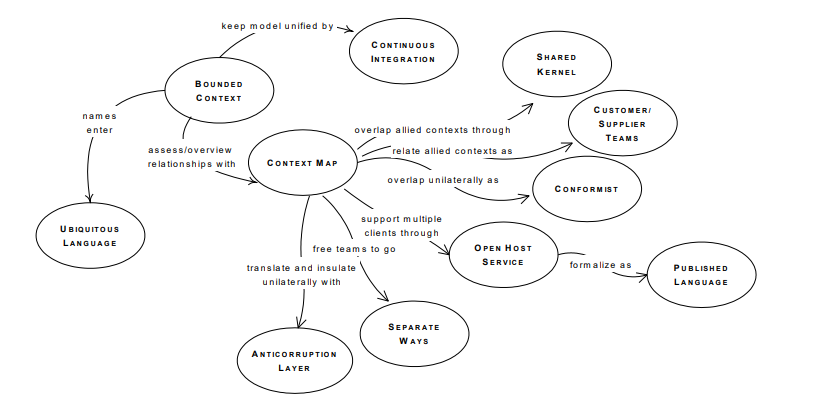
\includegraphics[scale = 0.9]{pictures/cac_mau_chien_luoc/temp.png}

\caption{Sơ đồ về các thành phần trong mẫu chiến lược}

\end{figure}

% !<! - - $ Vẽ lại sau khi trình bày xong các mục nhỏ - - >
\subsection{Miền phụ (Sub - Domain)}
Một miền kinh doanh lớn được tạo thành từ nhiều \emph{miền phụ (Sub - Domain)}. Trong thực tế, một miền kinh doanh phức tạp không thể có một chuyên gia miền có kiến thức về tất cả các miền phụ.

\begin{example} Trong miền thương mại điện tử lớn có thể có một số miền phụ sau:

\begin{itemize}

\item \textbf{Miền phụ quản lý hàng tồn kho:} liên quan đến việc quản lý sản phẩm trong kho hàng.

\item \textbf{Miền phụ quản lý khách hàng:} liên quan đến việc quản lý tài khoản khách hàng.

\item \textbf{Miền phụ vận chuyển:} liên quan đến việc quản lý việc vận chuyển giao hàng.

\end{itemize}

\end{example}

\subsubsection{Phân loại các miền phụ}

Trong thiết kế hướng miền, có ba loại miền phụ là:

\begin{itemize}

\item Miền phụ chung (Generic Subdomain)

Miền phụ chung cung cấp các giải pháp có sẵn mà doanh nghiệp có thể mua. Miền phụ chung có thể được tìm thấy trên nhiều ngành. Doanh nghiệp không thể đạt được bất kỳ lợi thế cạnh tranh so với đối thủ bằng cách thực hiện những điều khác biệt trong miền phụ chung.

\begin{example} Các miền phụ chung \emph{"quản lý nhân sự"} hay \emph{"quản lý cơ sở vật chất"} không tạo thêm bất kỳ giá trị khác biệt nào cho doanh nghiệp. \end{example}

\item Miền phụ cốt lõi (Core Subdomain)

Miền phụ cốt lõi là phần quan trọng và có giá trị nhất của hệ thống. Miền phụ cốt lõi giúp phân biệt các doanh nghiệp và làm cho các doanh nghiệp có giá trị. Miền phụ cốt lõi tập trung vào mục tiêu và yêu cầu của khách hàng với doanh nghiệp, từ đó quyết định sự thành công của doanh nghiệp. Vì vậy, mỗi doanh nghiệp luôn tìm cách thực hiện những điều khác biệt trong các miền phụ cốt lõi này để đạt được lợi thế so với đối thủ cạnh tranh.

\begin{example} Trong miền thẻ tín dụng, miền phụ cốt lõi có thể là \emph{"phát hành thẻ"} chịu trách nhiệm về quá trình phát hành thẻ tín dụng cho khách hàng. Miền phụ cốt lõi này bao gồm các nhiệm vụ như: thu thập thông tin khách hàng, thực hiện kiểm tra tín dụng, kích hoạt thẻ, \dots \end{example}

\item Miền phụ hỗ trợ (Supporting Subdomain)

Các miền phụ cốt lõi phụ thuộc vào các miền phụ hỗ trợ. Miền phụ hỗ trợ cung cấp các dịch vụ để miền phụ cốt lõi hoạt động hiệu quả. Tuy nhiên, miền phụ hỗ trợ không đòi hỏi mức độ phức tạp cao về logic nghiệp vụ.

\begin{example} Trong nhiều phần mềm, miền phụ hỗ trợ \emph{"xác thực người dùng"} OAuth 2.0 của Facebook hoặc Google hỗ trợ cho miền phụ cốt lõi hoạt động. \end{example}

\end{itemize}

\subsubsection{Cách xác định miền phụ}

Các miền phụ cốt lõi, hỗ trợ và chung có thể khác nhau đối với các doanh nghiệp vì tùy theo nhu cầu kinh doanh và bối cảnh cụ thể của mỗi tổ chức.

\textbf{Các bước xác định miền phụ:}

\begin{enumerate}

\item Bắt đầu bằng cách xem xét nghiệp vụ kinh doanh.

\item Nếu có sẵn giải pháp đã biết thì có khả năng là miền phụ chung. Ngược lại, chúng ta kiểm tra xem nghiệp vụ kinh doanh đó có thêm giá trị kinh doanh nào hay không?

\item Nếu không có giá trị kinh doanh thì chúng ta kiểm tra xem các miền phụ cốt lõi có phụ thuộc vào miền phụ này hay không? Nếu có thì có khả năng là miền phụ hỗ trợ. Nếu không thì đó là miền phụ chung.

\item Nếu miền phụ có tiềm năng bổ sung một số giá trị kinh doanh thì bước kiểm tra tiếp theo là xem liệu miền doanh nghiệp có độ phức tạp cao hay không?

\item Nếu miền doanh nghiệp không có độ phức tạp cao thì có khả năng là miền phụ hỗ trợ. Ngược lại thì nó có khả năng là miền phụ cốt lõi.

\end{enumerate}

\begin{figure}[H]

\centering


\includegraphics[scale = 0.5]{pictures/_so_do_xac_dinh_mien_phu/main.drawio.png}

\caption{Sơ đồ xác định miền phụ}

\end{figure}

\subsubsection{Áp dụng phân loại miền phụ trong đồ án này}

\begin{itemize}

\item Từ yêu cầu nghiệp vụ, em có thể phân chia thành các miền phụ như sau:

\begin{itemize}

\item Quản lý hóa đơn

\item Báo cáo thống kê

\item Thông báo

\item Thư điện tử

\item Quản lý hệ thống

\end{itemize}

\item Phân loại miền phụ

\begin{itemize}

\item Miền phụ chung

Có thể là các miền có sẵn, hoạt động ổn định, không được đề cập trong nghiệp vụ phần mềm hóa đơn điện tử như:

\begin{itemize}

\item Quản lý nhân sự

\item Quản lý cơ sở vật chất

\end{itemize}

\item Miền phụ cốt lõi

\begin{itemize}

\item Quản lý hóa đơn

Là miền cốt lõi quan trọng tạo lợi thế cạnh tranh trong ngành.

\item Báo cáo thống kê

Giúp theo dõi tình hình thông tin tài chính của doanh nghiệp.

\item Thông báo

Miền thông báo giúp hỗ trợ thông tin các quy định về thuế và pháp luật đến với khách hàng sử dụng.

\item Quản lý hệ thống

Miền này giúp xác thực và ủy quyền bảo vệ dữ liệu của khách hàng.

\end{itemize}

\item Miền phụ hỗ trợ

\item \begin{itemize}

\item Thư điện tử

Miền thư điện tử hỗ trợ miền cốt lõi trao đổi thông tin với khách hàng.

\end{itemize}

\end{itemize}

\end{itemize}
%@%%%%%%%%%%%%%%%%%%%%%%%%%%%% now()
\subsection{Ngôn ngữ chung (Ubiquitous Language)}
Trong quá trình hoạt động kinh doanh, không phải mọi doanh nghiệp đều giữ nguyên mô hình kinh doanh được đưa ra ban đầu. Việc chuyển đổi mô hình kinh doanh là điều cần thiết, giúp các doanh nghiệp có thể phát triển linh hoạt và tồn tại.
\begin{example}
    

\begin{itemize}

\item Google bắt đầu như công cụ tìm kiếm trực tuyến, nhưng sau đó đã mở rộng và thay đổi mô hình kinh doanh qua nhiều dịch vụ và sản phẩm khác nhau như: Dịch vụ đám mây Google Cloud Platform, Dịch vụ thư điện tử Gmail, Dịch vụ bản đồ Google Maps, Dịch vụ lưu trữ tập tin Google Drive, \dots

\item Amazon từ hiệu sách trực tuyến đã trở thành thị trường cho nhà cung cấp khác như: Thương mại điện tử, Dịch vụ đám mây Amazon Web Services (AWS), \dots

\end{itemize}
\end{example}
\begin{figure}[H]

\centering

\includegraphics[scale = 0.5]{pictures/kien_truc_vi_dich_vu_cua_amazon/main.png}

\caption{Kiến trúc vi dịch vụ của Amazon}

\end{figure}
%@%%%%%%%%%%%%%%%%%%%%%%%%%%%% now()

% Trong thời đại ngày nay, nhu cầu phát triển ứng dụng và hệ thống ngày càng tăng, đặt ra thách thức đối với kiến trúc phần mềm. Kiến trúc nguyên khối đã phục vụ hiệu quả trong quá khứ, nhưng kiến trúc này bắt đầu gặp khó khăn khi đối mặt với sự phức tạp, khả năng mở rộng và khả năng đáp ứng linh hoạt với sự thay đổi nhanh chóng trong yêu cầu kinh doanh.

% Kiến trúc vi dịch vụ là giải pháp cho những thách thức trên. Kiến trúc vi dịch vụ chia dự án thành những dịch vụ nhỏ độc lập, mỗi dịch vụ chịu trách nhiệm về một chức năng cụ thể. Từ đó, dự án giảm sự phức tạp, tăng tính linh hoạt và dễ dàng quản lý.

% Việc vận dụng kết hợp giữa kiến trúc vi dịch vụ và thiết kế hướng miền là một cách tiếp cận toàn diện, giúp xác định và tổ chức các dịch vụ dựa trên việc hiểu rõ về lĩnh vực kinh doanh. Thiết kế hướng miền xây dựng mô hình dựa trên yêu cầu nghiệp vụ thực tế, từ đó dự án phản ánh đúng các quy trình kinh doanh.

% Trong quá trình hoạt động kinh doanh, không phải mọi doanh nghiệp đều giữ nguyên mô hình kinh doanh được đưa ra ban đầu của mình. Khi quy mô thị trường thay đổi, việc chuyển đổi mô hình kinh doanh là điều cần thiết. Chuyển đổi kinh doanh như một công cụ linh hoạt giúp các doanh nghiệp có thể phát triển và tồn tại giữa các đối thủ của mình.




% Đối với những doanh nghiệp không chuyển đổi kinh doanh sẽ không thể tồn tại.

% \begin{example} Gần đây, dịch vụ giao đồ ăn Baemin đã rời khỏi thị trường Việt Nam cũng do sức ép từ các đối thủ khác khiến Baemin khó cạnh tranh trong mảng kinh doanh cốt lõi là giao đồ ăn. Các đối thủ này không chỉ cung cấp dịch vụ giao đồ ăn mà còn có đặt xe, giao hàng,...

% \end{example}

% \begin{figure}[H]

% \centering

% \includegraphics[scale = 0.5]{pictures/baemin/main.png}

% \caption{Dịch vụ giao đồ ăn Baemin đã rời khỏi thị trường Việt Nam}

% \end{figure}

% Hiện nay, các tổ chức doanh nghiệp có nhu cầu chuyển đổi kinh doanh để có thể tồn tại và phát triển khi thị trường thay đổi. Từ đó, đáp ứng nhu cầu của khách hàng, mang lại ưu thế cạnh tranh so với các đối thủ. Do đó, các doanh nghiệp cần hệ thống chuyển đổi nhanh chóng để đáp ứng nhu cầu của mô hình kinh doanh và mong đợi của khách hàng.

% Kiến trúc vi dịch vụ giải quyết những thách thức và hỗ trợ doanh nghiệp chuyển đổi kinh doanh, mở rộng hệ thống dễ dàng. Tuy nhiên, để xây dựng được một kiến trúc vi dịch vụ tốt, cần phải tạo ra các dịch vụ nhỏ phù hợp và duy trì tính độc lập. Trong đồ án này, em sử dụng thiết kế hướng miền để phân tích và xây dựng kiến trúc vi dịch vụ. Thiết kế hướng miền giúp xác định và tổ chức các dịch vụ dựa trên việc hiểu rõ về lĩnh vực kinh doanh, từ đó giúp dự án phản ánh chính xác các quy trình và quy tắc kinh doanh.


\subsection{Tích hợp liên tục (Continuous Integration)}
% Trong quá trình hoạt động kinh doanh, không phải mọi doanh nghiệp đều giữ nguyên mô hình kinh doanh được đưa ra ban đầu. Việc chuyển đổi mô hình kinh doanh là điều cần thiết, giúp các doanh nghiệp có thể phát triển linh hoạt và tồn tại.
\begin{example}
    

\begin{itemize}

\item Google bắt đầu như công cụ tìm kiếm trực tuyến, nhưng sau đó đã mở rộng và thay đổi mô hình kinh doanh qua nhiều dịch vụ và sản phẩm khác nhau như: Dịch vụ đám mây Google Cloud Platform, Dịch vụ thư điện tử Gmail, Dịch vụ bản đồ Google Maps, Dịch vụ lưu trữ tập tin Google Drive, \dots

\item Amazon từ hiệu sách trực tuyến đã trở thành thị trường cho nhà cung cấp khác như: Thương mại điện tử, Dịch vụ đám mây Amazon Web Services (AWS), \dots

\end{itemize}
\end{example}
\begin{figure}[H]

\centering

\includegraphics[scale = 0.5]{pictures/kien_truc_vi_dich_vu_cua_amazon/main.png}

\caption{Kiến trúc vi dịch vụ của Amazon}

\end{figure}
%@%%%%%%%%%%%%%%%%%%%%%%%%%%%% now()

% Trong thời đại ngày nay, nhu cầu phát triển ứng dụng và hệ thống ngày càng tăng, đặt ra thách thức đối với kiến trúc phần mềm. Kiến trúc nguyên khối đã phục vụ hiệu quả trong quá khứ, nhưng kiến trúc này bắt đầu gặp khó khăn khi đối mặt với sự phức tạp, khả năng mở rộng và khả năng đáp ứng linh hoạt với sự thay đổi nhanh chóng trong yêu cầu kinh doanh.

% Kiến trúc vi dịch vụ là giải pháp cho những thách thức trên. Kiến trúc vi dịch vụ chia dự án thành những dịch vụ nhỏ độc lập, mỗi dịch vụ chịu trách nhiệm về một chức năng cụ thể. Từ đó, dự án giảm sự phức tạp, tăng tính linh hoạt và dễ dàng quản lý.

% Việc vận dụng kết hợp giữa kiến trúc vi dịch vụ và thiết kế hướng miền là một cách tiếp cận toàn diện, giúp xác định và tổ chức các dịch vụ dựa trên việc hiểu rõ về lĩnh vực kinh doanh. Thiết kế hướng miền xây dựng mô hình dựa trên yêu cầu nghiệp vụ thực tế, từ đó dự án phản ánh đúng các quy trình kinh doanh.

% Trong quá trình hoạt động kinh doanh, không phải mọi doanh nghiệp đều giữ nguyên mô hình kinh doanh được đưa ra ban đầu của mình. Khi quy mô thị trường thay đổi, việc chuyển đổi mô hình kinh doanh là điều cần thiết. Chuyển đổi kinh doanh như một công cụ linh hoạt giúp các doanh nghiệp có thể phát triển và tồn tại giữa các đối thủ của mình.




% Đối với những doanh nghiệp không chuyển đổi kinh doanh sẽ không thể tồn tại.

% \begin{example} Gần đây, dịch vụ giao đồ ăn Baemin đã rời khỏi thị trường Việt Nam cũng do sức ép từ các đối thủ khác khiến Baemin khó cạnh tranh trong mảng kinh doanh cốt lõi là giao đồ ăn. Các đối thủ này không chỉ cung cấp dịch vụ giao đồ ăn mà còn có đặt xe, giao hàng,...

% \end{example}

% \begin{figure}[H]

% \centering

% \includegraphics[scale = 0.5]{pictures/baemin/main.png}

% \caption{Dịch vụ giao đồ ăn Baemin đã rời khỏi thị trường Việt Nam}

% \end{figure}

% Hiện nay, các tổ chức doanh nghiệp có nhu cầu chuyển đổi kinh doanh để có thể tồn tại và phát triển khi thị trường thay đổi. Từ đó, đáp ứng nhu cầu của khách hàng, mang lại ưu thế cạnh tranh so với các đối thủ. Do đó, các doanh nghiệp cần hệ thống chuyển đổi nhanh chóng để đáp ứng nhu cầu của mô hình kinh doanh và mong đợi của khách hàng.

% Kiến trúc vi dịch vụ giải quyết những thách thức và hỗ trợ doanh nghiệp chuyển đổi kinh doanh, mở rộng hệ thống dễ dàng. Tuy nhiên, để xây dựng được một kiến trúc vi dịch vụ tốt, cần phải tạo ra các dịch vụ nhỏ phù hợp và duy trì tính độc lập. Trong đồ án này, em sử dụng thiết kế hướng miền để phân tích và xây dựng kiến trúc vi dịch vụ. Thiết kế hướng miền giúp xác định và tổ chức các dịch vụ dựa trên việc hiểu rõ về lĩnh vực kinh doanh, từ đó giúp dự án phản ánh chính xác các quy trình và quy tắc kinh doanh.



\subsection{Bối cảnh bị giới hạn (Bounded Context)}
\subsection{Mối quan hệ bối cảnh bị giới hạn (Bounded Context Relationships)}
\subsection{Bản đồ bối cảnh (Context Maps)}
%%%%%%%%%%%%%%%%%%%%%%%%%%%%%%
% Trong quá trình hoạt động kinh doanh, không phải mọi doanh nghiệp đều giữ nguyên mô hình kinh doanh được đưa ra ban đầu. Việc chuyển đổi mô hình kinh doanh là điều cần thiết, giúp các doanh nghiệp có thể phát triển linh hoạt và tồn tại.
\begin{example}
    

\begin{itemize}

\item Google bắt đầu như công cụ tìm kiếm trực tuyến, nhưng sau đó đã mở rộng và thay đổi mô hình kinh doanh qua nhiều dịch vụ và sản phẩm khác nhau như: Dịch vụ đám mây Google Cloud Platform, Dịch vụ thư điện tử Gmail, Dịch vụ bản đồ Google Maps, Dịch vụ lưu trữ tập tin Google Drive, \dots

\item Amazon từ hiệu sách trực tuyến đã trở thành thị trường cho nhà cung cấp khác như: Thương mại điện tử, Dịch vụ đám mây Amazon Web Services (AWS), \dots

\end{itemize}
\end{example}
\begin{figure}[H]

\centering

\includegraphics[scale = 0.5]{pictures/kien_truc_vi_dich_vu_cua_amazon/main.png}

\caption{Kiến trúc vi dịch vụ của Amazon}

\end{figure}
%@%%%%%%%%%%%%%%%%%%%%%%%%%%%% now()

% Trong thời đại ngày nay, nhu cầu phát triển ứng dụng và hệ thống ngày càng tăng, đặt ra thách thức đối với kiến trúc phần mềm. Kiến trúc nguyên khối đã phục vụ hiệu quả trong quá khứ, nhưng kiến trúc này bắt đầu gặp khó khăn khi đối mặt với sự phức tạp, khả năng mở rộng và khả năng đáp ứng linh hoạt với sự thay đổi nhanh chóng trong yêu cầu kinh doanh.

% Kiến trúc vi dịch vụ là giải pháp cho những thách thức trên. Kiến trúc vi dịch vụ chia dự án thành những dịch vụ nhỏ độc lập, mỗi dịch vụ chịu trách nhiệm về một chức năng cụ thể. Từ đó, dự án giảm sự phức tạp, tăng tính linh hoạt và dễ dàng quản lý.

% Việc vận dụng kết hợp giữa kiến trúc vi dịch vụ và thiết kế hướng miền là một cách tiếp cận toàn diện, giúp xác định và tổ chức các dịch vụ dựa trên việc hiểu rõ về lĩnh vực kinh doanh. Thiết kế hướng miền xây dựng mô hình dựa trên yêu cầu nghiệp vụ thực tế, từ đó dự án phản ánh đúng các quy trình kinh doanh.

% Trong quá trình hoạt động kinh doanh, không phải mọi doanh nghiệp đều giữ nguyên mô hình kinh doanh được đưa ra ban đầu của mình. Khi quy mô thị trường thay đổi, việc chuyển đổi mô hình kinh doanh là điều cần thiết. Chuyển đổi kinh doanh như một công cụ linh hoạt giúp các doanh nghiệp có thể phát triển và tồn tại giữa các đối thủ của mình.




% Đối với những doanh nghiệp không chuyển đổi kinh doanh sẽ không thể tồn tại.

% \begin{example} Gần đây, dịch vụ giao đồ ăn Baemin đã rời khỏi thị trường Việt Nam cũng do sức ép từ các đối thủ khác khiến Baemin khó cạnh tranh trong mảng kinh doanh cốt lõi là giao đồ ăn. Các đối thủ này không chỉ cung cấp dịch vụ giao đồ ăn mà còn có đặt xe, giao hàng,...

% \end{example}

% \begin{figure}[H]

% \centering

% \includegraphics[scale = 0.5]{pictures/baemin/main.png}

% \caption{Dịch vụ giao đồ ăn Baemin đã rời khỏi thị trường Việt Nam}

% \end{figure}

% Hiện nay, các tổ chức doanh nghiệp có nhu cầu chuyển đổi kinh doanh để có thể tồn tại và phát triển khi thị trường thay đổi. Từ đó, đáp ứng nhu cầu của khách hàng, mang lại ưu thế cạnh tranh so với các đối thủ. Do đó, các doanh nghiệp cần hệ thống chuyển đổi nhanh chóng để đáp ứng nhu cầu của mô hình kinh doanh và mong đợi của khách hàng.

% Kiến trúc vi dịch vụ giải quyết những thách thức và hỗ trợ doanh nghiệp chuyển đổi kinh doanh, mở rộng hệ thống dễ dàng. Tuy nhiên, để xây dựng được một kiến trúc vi dịch vụ tốt, cần phải tạo ra các dịch vụ nhỏ phù hợp và duy trì tính độc lập. Trong đồ án này, em sử dụng thiết kế hướng miền để phân tích và xây dựng kiến trúc vi dịch vụ. Thiết kế hướng miền giúp xác định và tổ chức các dịch vụ dựa trên việc hiểu rõ về lĩnh vực kinh doanh, từ đó giúp dự án phản ánh chính xác các quy trình và quy tắc kinh doanh.


%%%%%%%%%%%%%%%%%%%%%%%%%%%%%%

%#%%%%%%%%%%%%%%%%%%%%%%%%%%%%
%#%%%%%%%%%%%%%%%%%%%%%%%%%%%%
%#%%%%%%%%%%%%%%%%%%%%%%%%%%%%
%#%%%%%%%%%%%%%%%%%%%%%%%%%%%%
%#%%%%%%%%%%%%%%%%%%%%%%%%%%%%
%#%%%%%%%%%%%%%%%%%%%%%%%%%%%%
%#%%%%%%%%%%%%%%%%%%%%%%%%%%%%
%#%%%%%%%%%%%%%%%%%%%%%%%%%%%%
%#%%%%%%%%%%%%%%%%%%%%%%%%%%%%
%#%%%%%%%%%%%%%%%%%%%%%%%%%%%%
%#%%%%%%%%%%%%%%%%%%%%%%%%%%%%
%#%%%%%%%%%%%%%%%%%%%%%%%%%%%%
%#%%%%%%%%%%%%%%%%%%%%%%%%%%%%
%#%%%%%%%%%%%%%%%%%%%%%%%%%%%%
%#%%%%%%%%%%%%%%%%%%%%%%%%%%%%
%#%%%%%%%%%%%%%%%%%%%%%%%%%%%%
\section{Các mẫu kỹ thuật trong thiết kế hướng miền}
% \section{Đối tượng miền (Domain Object)}
% \subsection{Đối tượng thực thể (Entities Objects)}
% % \subsection{Đối tượng thực thể (Entities Objects)}
% \subsection{Đối tượng giá trị (Value Objects)}
% \subsection{Miền dịch vụ (Service Domain)}

% \subsubsection{Phân loại các miền phụ}
% \subsubsection{Cách xác định các miền phụ}
% % \subsubsection{Mô tả cách xác định các miền phụ}
% % \section{Mô hình miền (Domain Models)}
% % \section{Bối cảnh bị giới hạn (Bounded Context)}
% \subsubsection{Cách xác định bối cảnh bị giới hạn}
% \subsubsection{Áp dụng xác định bối cảnh bị giới hạn trong đồ án này}
% % \section{Ngôn ngữ chung (Ubiquitous Language)}
% \subsubsection{Một số đặc điểm của ngôn ngữ chung}
% % \section{Bản đồ bối cảnh (Context Maps)}
% % \section{Các mối quan hệ bối cảnh bị giới hạn}
% % \subsection{Mối quan hệ đối xứng (Symmetric Relationship)}
% % \subsubsection{Mô hình riêng biệt (Separate Ways)}
% % \subsubsection{Mô hình hạt nhân chung (Shared Kernel)}
% % \subsection{Mối quan hệ bất đối xứng (Asymmetric Relationship)}
% % \subsubsection{Mô hình khách hàng - nhà cung cấp (Customer - Supplier)}
% % \subsubsection{Mô hình tuân thủ (Conformist)}
% % \subsubsection{Mô hình chống đổ vỡ (Anti Corruption Layer)}
% % \subsection{Mối quan hệ 1 - nhiều (One to Many Relationship)}
% % \subsubsection{Dịch vụ máy chủ mở (Open Host Service)}
% % \subsubsection{Ngôn ngữ được xuất bản (Published Language)}
% % \section{Áp dụng về các mối quan hệ bối cảnh bị giới hạn}
% \section{Đối tượng miền (Domain Object)}
% \subsection{Đối tượng thực thể (Entities Objects)}
% % \subsection{Đối tượng thực thể (Entities Objects)}
% \subsection{Đối tượng giá trị (Value Objects)}
% \subsection{Miền dịch vụ (Service Domain)}
% % \subsubsection{xxxxxxx}
% % \subsubsection{xxxxxxx}
\end{document}
%#%%%%%%%%%%%%%%%%%%%%%%%%%%%%
%%%%%%%%%%%%%%%%%%%%%%%%%%%%%%
%%%%%%%%%%%%%%%%%%%%%%%%%%%%%%
%%%%%%%%%%%%%%%%%%%%%%%%%%%%%%
%%%%%%%%%%%%%%%%%%%%%%%%%%%%%%
%%%%%%%%%%%%%%%%%%%%%%%%%%%%%%
%%%%%%%%%%%%%%%%%%%%%%%%%%%%%%
%%%%%%%%%%%%%%%%%%%%%%%%%%%%%%
%%%%%%%%%%%%%%%%%%%%%%%%%%%%%%
%%%%%%%%%%%%%%%%%%%%%%%%%%%%%%
%# Một số công nghệ trong kiến trúc vi dịch vụ
%# Một số công nghệ trong kiến trúc vi dịch vụ
%# Một số công nghệ trong kiến trúc vi dịch vụ
%# Một số công nghệ trong kiến trúc vi dịch vụ
%# Một số công nghệ trong kiến trúc vi dịch vụ
%# Một số công nghệ trong kiến trúc vi dịch vụ
%# Một số công nghệ trong kiến trúc vi dịch vụ
%# Một số công nghệ trong kiến trúc vi dịch vụ
%# Một số công nghệ trong kiến trúc vi dịch vụ
%# Một số công nghệ trong kiến trúc vi dịch vụ
%# Một số công nghệ trong kiến trúc vi dịch vụ
%# Một số công nghệ trong kiến trúc vi dịch vụ
%# Một số công nghệ trong kiến trúc vi dịch vụ
%# Một số công nghệ trong kiến trúc vi dịch vụ
%# Một số công nghệ trong kiến trúc vi dịch vụ
%# Một số công nghệ trong kiến trúc vi dịch vụ
%# Một số công nghệ trong kiến trúc vi dịch vụ
%# Một số công nghệ trong kiến trúc vi dịch vụ
%# Một số công nghệ trong kiến trúc vi dịch vụ
%# Một số công nghệ trong kiến trúc vi dịch vụ
%# Một số công nghệ trong kiến trúc vi dịch vụ
%# Một số công nghệ trong kiến trúc vi dịch vụ
%# Một số công nghệ trong kiến trúc vi dịch vụ
%# Một số công nghệ trong kiến trúc vi dịch vụ
%# Một số công nghệ trong kiến trúc vi dịch vụ
%# Một số công nghệ trong kiến trúc vi dịch vụ
%# Một số công nghệ trong kiến trúc vi dịch vụ
%# Một số công nghệ trong kiến trúc vi dịch vụ
%# Một số công nghệ trong kiến trúc vi dịch vụ
%#%%%%%%%%%%%%%%%%%%%%%%%%%%%%
\chapter{Một số công nghệ trong kiến trúc vi dịch vụ}
% % \section{xxxxxxxxxxxxxxxxxx}

% % phải có CQRS (Phân chia trách nhiệm truy vấn lệnh)

% CQRS là một mẫu kiến trúc riêng biệt có thể được sử dụng kết hợp với thiết kế hướng miền để đạt được những lợi ích nhất định, chẳng hạn như cải thiện hiệu suất và khả năng mở rộng. Tuy nhiên, nó không phải là một yêu cầu để triển khai thiết kế hướng miền.

% % phải có event

% Cách tiếp cận này nhấn mạnh tính mô - đun, tính linh hoạt và khả năng phục hồi, cho phép các nhóm làm việc đồng thời trên các phần khác nhau của hệ thống và cho phép phát hành nhanh hơn và thường xuyên hơn. Các vi dịch vụ thường dựa vào các giao thức truyền thông nhẹ, chẳng hạn như REST và thường được triển khai bằng các công nghệ chứa trong bộ chứa như Docker và Kubernetes.

% \subsubsection{DevOps Ứng dụng, áp dụng, liên quan,....}

% \subsubsection{Github}

% \subsubsection{CI/CD}

% \subsubsection{Docker}

% \subsubsection{Kubernetes}

% dícovery

% % api gateway

% Repository độc lập miền và lưu trữ sql (dễ tuhaajn tiện Unit testing and Mocking)

% Repository trong ORM

% <!--https: //images.viblo.asia/fd4b10a0-f1b1-4ed1-9bd1-578c871820ae.png-->

% , gprc rabitmq đồng bộ hay k, ít hay nhiều như pub sub

% # 5. Service Mesh, CICD, microfe, API gateway, cache redis, log xử lí lỗi,

% <!---->

% Bảng CSDL này được em thu thập dữ liệu từ trang web CƠ SỞ DỮU DANH MỤC DÙNG CHUNG (https: //dmdc.mof.gov.vn/khai-thac-pb/co-quan-thue)

% https: //helpsme.misa.vn/2020/kb/quan-ly-hoa-don-dien-tu/

% https: //helpsme.misa.vn/2022/kb/quy-trinh-nghiep-vu-hddt-theo-nghi-dinh-123-2020-nd-cp/

% https: //www.meinvoice.vn/tin-tuc/3442/nhung-nghiep-vu-co-ban-cua-hoa-don-dien-tu-xac-thuc/

% <!---->

% Bảng CSDL này được em thu thập dữ liệu từ trang web CƠ SỞ DỮU DANH MỤC DÙNG CHUNG (https: //dmdc.mof.gov.vn/khai-thac-pb/co-quan-thue)

% https: //helpsme.misa.vn/2020/kb/quan-ly-hoa-don-dien-tu/

% https: //helpsme.misa.vn/2022/kb/quy-trinh-nghiep-vu-hddt-theo-nghi-dinh-123-2020-nd-cp/

% https: //www.meinvoice.vn/tin-tuc/3442/nhung-nghiep-vu-co-ban-cua-hoa-don-dien-tu-xac-thuc/

% <!--Thay thế = NULL-->

% <!--Bị thay thế = NULL-->

% <!--quy trình tương tự như lập mới hóa đơn giá trị gia tăng.-->

% <!---->

% <!--@Chú ý ở đồ án này:-->

% <!--Sử dụng hàm ngẫu nhiên (tỉ lệ 10%) cho trường hợp "Mã số thuế không tồn tại."-->

% <!--Sử dụng hàm ngẫu nhiên tạo tên cho Tên NNT vì em không có thông tin đăng ký thực tế của NNT.-->

% <!--Sử dụng hàm ngẫu nhiên trong bảng CSDL cho "Mã cơ quan thuế quản lý" và "Tên cơ quan thuế quản lý"-->

% Bảng CSDL này được em thu thập dữ liệu từ trang web CƠ SỞ DỮU DANH MỤC DÙNG CHUNG (https: //dmdc.mof.gov.vn/khai-thac-pb/co-quan-thue)

% <!--!Mã thuế số-chi nhánh-->

% <!--Mã captcha không đúng.-->

% <!--0107001729-->

% dấu chấm cuối câu .

% email=>Thư điện tử

% Viết tắt NNT...

% <!--Validtae-->

% Điều kiện

% <!---->

% Chỉ dùng 1 loại hóa đơn vì em thấy tương tự.

% Loại hóa đơn: + Hóa đơn giá trị gia tăng + Hóa đơn bán hàng + Hóa đơn bán tài sản công + Hóa đơn bán hàng dự trữ quốc gia + Hóa đơn khác + Chứng từ điện tử được sử dụng và quản lý như hóa đơn

% <!--Nghiệp vụ của bài toán chính-->

% Video Viettel

% <!--@Chú ý ở đồ án này:-->

% Mã giao dịch điện tử = Mã số thuế + Thời gian đăng kí

% Sử dụng hàm ngẫu nhiên (tỉ lệ 10%) cho trường hợp từ chối.

% <!--Phân tích và thiết kế-->

% Xác định các tính năng cần thiết và các yêu cầu kỹ thuật tạo ra một thiết kế hệ thống hoặc kiến trúc đáp ứng.

% <!---->

% <!--Các công nghệ phổ biến trong kiến trúc vi dịch vụ-->

% Docker container.....

% Docker container.....

% Docker container.....

% Docker container.....

% [](0.9.KetLuan_TongKet.md)

% [](_.TaiLieuThamKhao.md)

% <!--RxJS-->

% https: //www.youtube.com/watch? v=6jSk_J7RA24

% https: //www.youtube.com/watch? v=Jc-lGeDuphg

% https: //www.youtube.com/watch? v=UXHzxX4png0

% https: //www.youtube.com/watch? v=glZs4QFfwbc

% # 6. Container và Container Orchestration

% Docker and Kubernetes (often abbreviated as K8s) are two powerful technologies commonly used in the world of container orchestration and deployment. Let's briefly explore each of them:

% 1. **Docker: **

% - **Containerization Technology: ** Docker is a platform that enables developers to automate the deployment of applications inside lightweight, portable containers. Containers encapsulate an application and its dependencies, ensuring consistency across different environments.

% - **Docker Image: ** A Docker image is a lightweight, standalone, executable package that includes everything needed to run a piece of software, including the code, runtime, libraries, and system tools.

% - **Docker Container: ** An instance of a Docker image is called a Docker container. Containers run consistently across different environments, providing a consistent and reproducible runtime.

% 2. **Kubernetes (K8s): **

% - **Container Orchestration: ** Kubernetes is an open-source container orchestration platform that automates the deployment, scaling, and management of containerized applications. It abstracts the underlying infrastructure and provides a unified API to manage clusters of containers.

% - **Key Concepts: ** Kubernetes introduces concepts like Pods (smallest deployable units), Deployments (managing replica sets and rolling updates), Services (networking abstraction for pods), and more.

% - **Scaling and Load Balancing: ** Kubernetes can scale applications horizontally by adding or removing instances (pods) based on demand. It also provides load balancing to distribute traffic across multiple instances.

% **How Docker and Kubernetes Work Together: **

% - Docker is used to create containerized applications, and Kubernetes manages the orchestration of these containers.

% - Developers package their applications into Docker containers, which can run locally on a developer's machine.

% - Kubernetes then takes these containers and orchestrates their deployment, ensuring high availability, scalability, and easy management.

% **Common Commands: **

% - **Docker Commands: **

% - `docker build`: Build a Docker image from a Dockerfile.

% - `docker run`: Create and start a Docker container.

% - `docker push`: Push a Docker image to a registry.

% - **Kubernetes Commands: **

% - `kubectl apply`: Apply configurations to a cluster.

% - `kubectl get`: Display information about resources.

% - `kubectl describe`: Show detailed information about a resource.

% - `kubectl scale`: Scale the number of replicas in a deployment.

% **Integration: **

% - Docker images are often stored in container registries like Docker Hub.

% - Kubernetes can pull these Docker images from a registry and deploy them onto the cluster.

% In summary, Docker is used to containerize applications, and Kubernetes is used to orchestrate and manage these containers in a production environment. Together, they provide a powerful and scalable solution for deploying and managing containerized applications.

% # 7. Broker Pattern dịch vụ dicovery

% https: //www.youtube.com/watch? v=UXHzxX4png0

% # 8. Dependency Injection

% # 9. Kết luận tổng kết

% Kiến trúc vi dịch vụ, với việc tách biệt hệ thống thành các thành phần nhỏ quản lý độc lập, mang lại tính linh hoạt và khả năng mở rộng.

% thiết kế hướng miền giúp xây dựng mô hình chính xác và nhất quán của lĩnh vực kinh doanh, giúp đảm bảo rằng hệ thống phản ánh đúng yêu cầu nghiệp vụ.

% <!--@============================================== -->

% <!--@============================================== -->

% <!--@============================================== -->

% <!--@============================================== -->

% <!--@============================================== -->

% <!--@============================================== -->

% <!--@============================================== -->

% <!--@============================================== -->

% <!--@============================================== -->

% <!--@============================================== -->

% <!--@============================================== -->

% <!--@saga -->

% <!--@saga -->

% <!--@saga -->

% <!--@saga -->

% <!--@saga -->

% <!--@saga -->

% <!--@saga -->

% <!--@saga -->

% <!--@saga -->

% <!--@saga -->

% <!--@saga -->

% <!--@saga -->

% <!--@saga -->

% <!--@saga -->

% <!--@saga -->

% <!--@saga -->

% <!--@saga -->

% <!--@saga -->

% <!--@saga -->

% <!--@saga -->

% <!---->

% <!--!-->

% <!--@CQRS (Command Query Responsibility Segregation): -->

% <!--CQRS, EventSourcing, Sagas-->

% <!--@Event Sourcing: -->

% <!-- Strong Consistency : https://ddd-practitioners.com/?page_id=421 -->

% <!-- Snapshots : https://ddd-practitioners.com/snapshots -->

% <!-- Saga : https://ddd-practitioners.com/home/glossary/saga -->

% <!-- Outbox Pattern -->

% <!-- Optimistic Concurrency Control : https://ddd-practitioners.com/?page_id=609 -->

% <!-- https://www.linkedin.com/pulse/api-strategy-conways-law-inverse-conway-manoeuvre-mikael-wall%C3%A9n/ -->

% Một mô hình lưu trữ dữ liệu, trong đó tất cả các thay đổi trạng thái của hệ thống được biểu diễn dưới dạng sự kiện (event).

% <!-- EventStorming : https://ddd-practitioners.com/home/glossary/eventstorming -->

% <!-- Domain Storytelling : https://ddd-practitioners.com/?page_id=1005 -->

% <!-- CQRS : https://ddd-practitioners.com/?page_id=574 -->

% CQRS chia để thoải mái, chặt chẽ

% Là một nguyên tắc trong DDD, CQRS tách biệt giữa phần xử lý câu lệnh (Command) và phần truy vấn dữ liệu (Query).

% Command đại diện cho các thao tác cập nhật dữ liệu, trong khi Query đại diện cho các thao tác truy vấn dữ liệu.

% <!-- Event-Driven Architecture : https://ddd-practitioners.com/home/glossary/event-driven-architecture -->

% <!-- Event Modeling : https://ddd-practitioners.com/?page_id=994 -->

% <!-- Event Replay : https://ddd-practitioners.com/?page_id=585 -->

% <!-- Event Sourced Aggregates : https://ddd-practitioners.com/event-sourcing -->

% <!-- Event Sourcing : https://ddd-practitioners.com/?page_id=581 -->

% <!-- Eventual Consistency : https://ddd-practitioners.com/?page_id=419 -->

% <!-- Change Data Capture: https://en.wikipedia.org/wiki/CAP_theorem -->

% <!-- ACID Transaction : https://ddd-practitioners.com/?page_id=415 -->

% ACID (Atomicity, Consistency, Isolation, Durability)

% <!-- BASE Transaction -->

% BASE là viết tắt của "Basically Available, Soft state, Eventually consistent," và đối lập với ACID

% <!-- Command : https://ddd-practitioners.com/?page_id=596 -->

% <!-- Command Handler : https://ddd-practitioners.com/?page_id=599 -->

% <!-- Compensating Action : https://ddd-practitioners.com/compensating-action -->

% <!-- Compensating Transaction : https://ddd-practitioners.com/compensating-transaction -->

% <!-- Compensating Workflow : https://ddd-practitioners.com/compensating-workflow -->

% <!-- Domain Event : https://ddd-practitioners.com/domain-event -->

% <!--@ Dependency Inversion Principle -->

% SOLID : https://ddd-practitioners.com/home/glossary/solid

% Single Responsibility Principle : https://ddd-practitioners.com/single-responsibility-principle

% Open-Closed Principle

% Liskov Substitution Principle : https://ddd-practitioners.com/home/glossary/liskov-substitution-principle

% Interface Segregation Principle : https://ddd-practitioners.com/?page_id=817

% <!--!========================================================== -->

% <!--!========================================================== -->

% <!--!========================================================== -->

% <!--!========================================================== -->

% <!--!========================================================== -->

% <!--!========================================================== -->

% <!--!========================================================== -->

% <!-- mỗi dịch vụ xuất bản và đăng ký các sự kiện nếu cần. Cách tiếp cận này có thể mở rộng và linh hoạt hơn so với điều phối, nhưng cũng phức tạp hơn trong việc triển khai và bảo trì. Tuy nhiên, nó cũng có thể linh hoạt hơn vì mỗi dịch vụ có thể phát triển độc lập và lỗi trong một dịch vụ không nhất thiết ảnh hưởng đến toàn bộ hệ thống. -->

% <!-- PublishSubscribe : https://www.enterpriseintegrationpatterns.com/patterns/messaging/PublishSubscribeChannel.html -->

% <!--@gRPC -->

% <!--@gRPC -->

% <!--@gRPC -->

% <!--@gRPC -->

% <!--@gRPC -->

% <!--@gRPC -->

% <!--@gRPC -->

% <!--@gRPC -->

% <!--@gRPC -->

% <!--@gRPC -->

% <!--@gRPC -->

% % Để phát triển tốt

% % cần tạo một bộ kiểm thử tích hợp tự động

% CI/CD đã trình bày bên trên

% % nhằm kiểm tra tính đúng đắn

% % %! Test - Driven Development : https:// thiết kế hướng miền - practitioners.com/test - driven - development

% % %! Test - Driven Development : https:// thiết kế hướng miền - practitioners.com/test - driven - development

% % %! Test - Driven Development : https:// thiết kế hướng miền - practitioners.com/test - driven - development

% % %! Test - Driven Development : https:// thiết kế hướng miền - practitioners.com/test - driven - development

% % %! Test - Driven Development : https:// thiết kế hướng miền - practitioners.com/test - driven - development

% [[Test - Driven Development]] TDD is a lightweight programming methodology that emphasizes fast, incremental development and especially writing tests before writing code. Ideally these follow one another in cycles measured in minutes. (see full definition under [[Test - Driven Development]] topic)

% Trang chủTrang chủBảng chú giảiHướng phát triển thử nghiệm

% Hướng phát triển thử nghiệm

% Phát triển dựa trên thử nghiệm (TDD) là một phương pháp phát triển phần mềm trong đó các thử nghiệm được viết trước khi mã thực tế được phát triển. Mục đích của TDD là đảm bảo rằng mỗi đoạn mã đều được kiểm tra đầy đủ và đáp ứng các yêu cầu của doanh nghiệp. TDD liên quan đến việc viết một bài kiểm tra thất bại trước tiên, viết mã vừa đủ để vượt qua, sau đó tái cấu trúc mã để cải thiện thiết kế của nó trong khi vẫn đảm bảo rằng tất cả các bài kiểm tra đều vượt qua.

% TDD là một phương pháp quan trọng trong Thiết kế hướng miền (thiết kế hướng miền) vì nó giúp đảm bảo rằng mã được phát triển phù hợp với mô hình miền và các quy tắc miền. Bằng cách viết bài kiểm tra trước, nhà phát triển buộc phải suy nghĩ về mô hình miền và các quy tắc miền trước khi viết bất kỳ mã nào. Các thử nghiệm trở thành một cách để xác định hành vi của hệ thống và giúp tập trung vào các yêu cầu kinh doanh. Khi mã được phát triển và tái cấu trúc, các thử nghiệm sẽ đảm bảo rằng hệ thống vẫn phù hợp với mô hình miền và các yêu cầu kinh doanh.

% % %! Test - Driven Development : https:// thiết kế hướng miền - practitioners.com/test - driven - development

% % %! Test - Driven Development : https:// thiết kế hướng miền - practitioners.com/test - driven - development

% % %! Test - Driven Development : https:// thiết kế hướng miền - practitioners.com/test - driven - development

% % %! Test - Driven Development : https:// thiết kế hướng miền - practitioners.com/test - driven - development

\end{document}
%#%%%%%%%%%%%%%%%%%%%%%%%%%%%%
%!%%%%%%%%%%%%%%%%%%%%%%%%%%%%
%!%%%%%%%%%%%%%%%%%%%%%%%%%%%%
%!%%%%%%%%%%%%%%%%%%%%%%%%%%%%
%!%%%%%%%%%%%%%%%%%%%%%%%%%%%%
%!%%%%%%%%%%%%%%%%%%%%%%%%%%%%
%!%%%%%%%%%%%%%%%%%%%%%%%%%%%%
%!%%%%%%%%%%%%%%%%%%%%%%%%%%%%
%!%%%%%%%%%%%%%%%%%%%%%%%%%%%%
%!%%%%%%%%%%%%%%%%%%%%%%%%%%%%
%!%%%%%%%%%%%%%%%%%%%%%%%%%%%%
%!%%%%%%%%%%%%%%%%%%%%%%%%%%%%
%!%%%%%%%%%%%%%%%%%%%%%%%%%%%%
%!%%%%%%%%%%%%%%%%%%%%%%%%%%%%
%!%%%%%%%%%%%%%%%%%%%%%%%%%%%%
%!%%%%%%%%%%%%%%%%%%%%%%%%%%%%
%!%%%%%%%%%%%%%%%%%%%%%%%%%%%%
%!%%%%%%%%%%%%%%%%%%%%%%%%%%%%
%!%%%%%%%%%%%%%%%%%%%%%%%%%%%%
\end{document} % Kết thúc
%%%%%%%%%%%%%%%%%%%%%%%%%%%%%%
%%%%%%%%%%%%%%%%%%%%%%%%%%%%%%
%%%%%%%%%%%%%%%%%%%%%%%%%%%%%%